\chapter{数据库存储}

\begin{introduction}[期末考试提纲]
    \item RAID1、RAID5定义及其特性, 所适用的数据库应用场合
    \item 数据库的页结构和行结构
    \item LSM树、B+树
    \item 位图索引、按列存储
\end{introduction}

\section{存储介质}

这部分的内容也可以看操作系统的教材《Operating Systems: Three Easy Pieces》\cite{ArpaciDusseau23-Book}.

\begin{figure}[H]
    \centering
    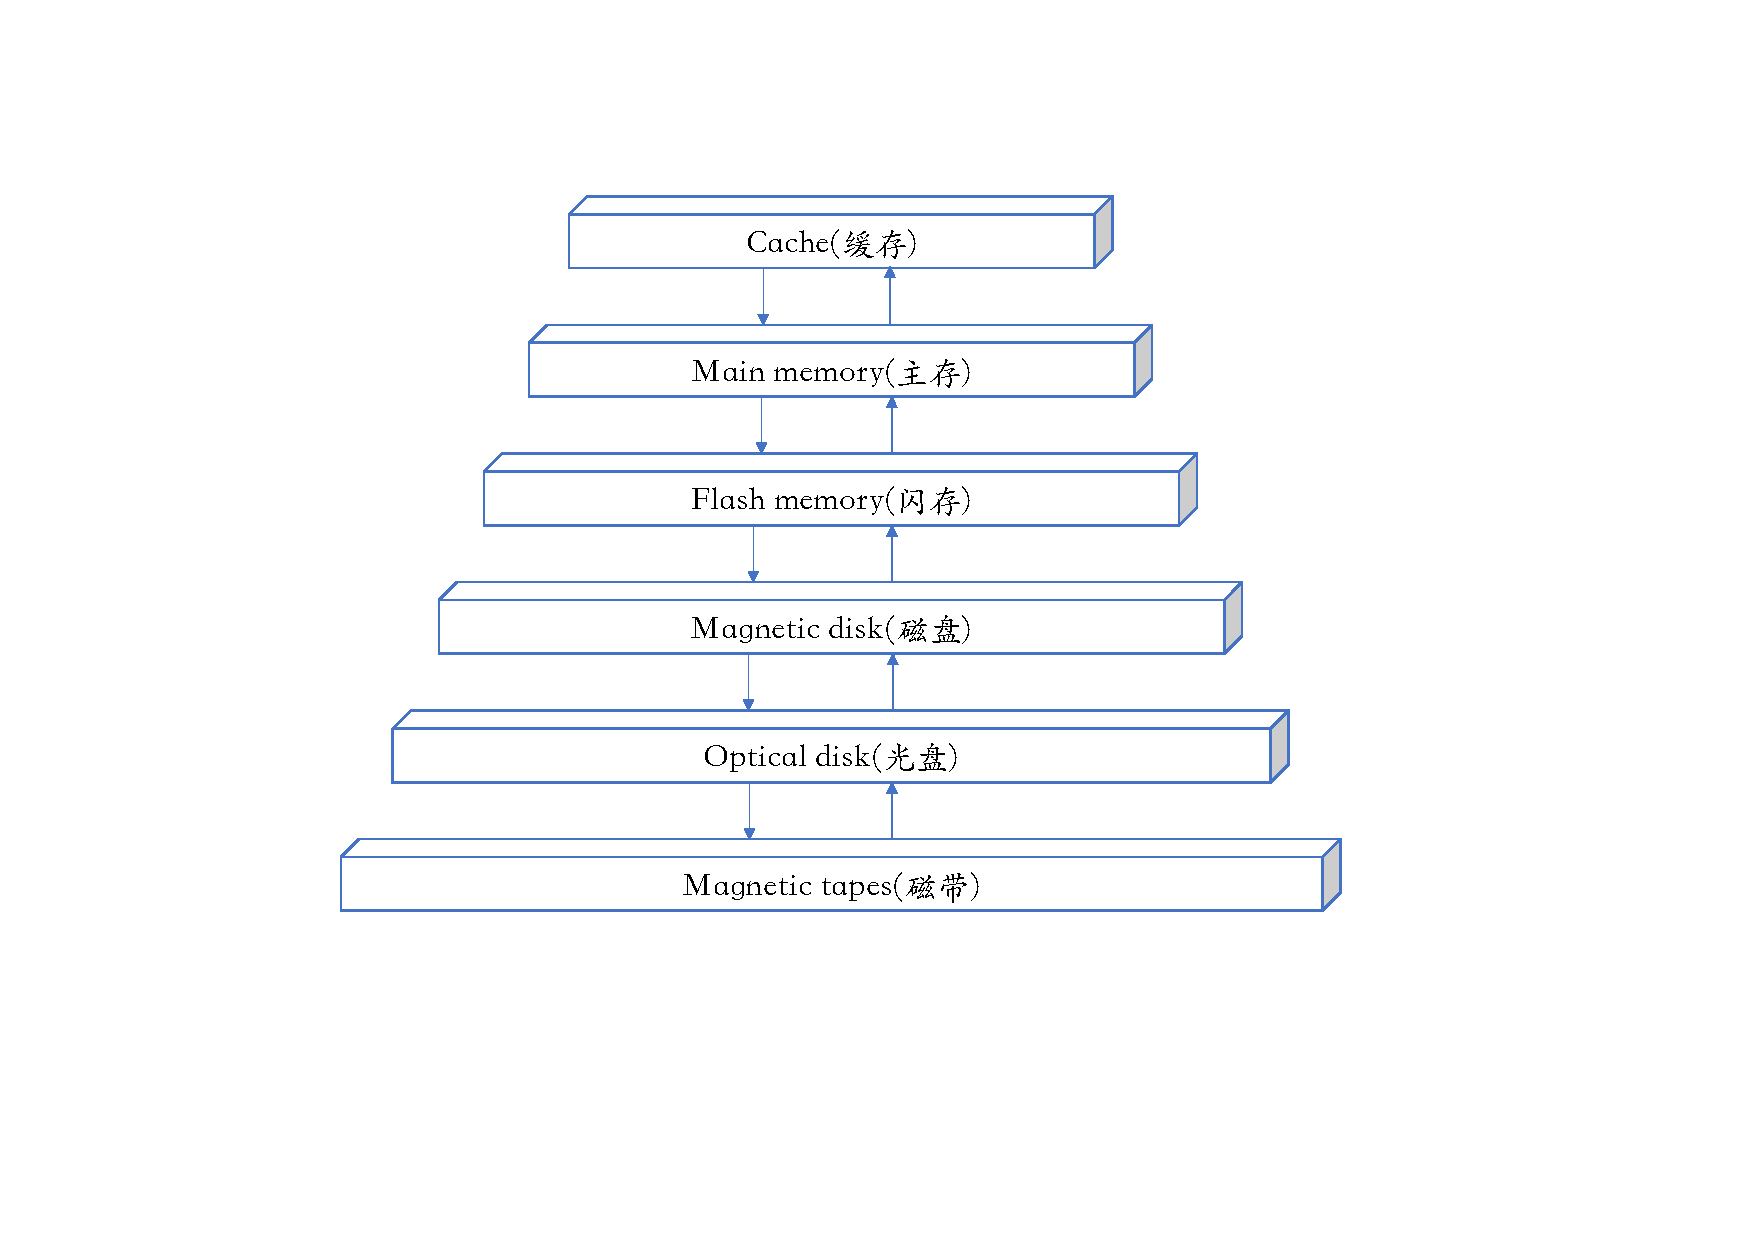
\includegraphics[width=.65\textwidth]{./figure/存储介质层次.pdf}
    \caption{物理存储介质的层次}
\end{figure}

局部性原理: CPU访问存储器时, 无论是存取指令还是存取数据, 所访问的存储单元都趋于聚集在一个较小的连续区域中.

\begin{itemize}
    \item 高速缓冲存储器(Cache): 最快最昂贵的存储介质; 很小, 由操作系统管理.
    \item 主存储器(main memory): 存放可被处理的数据的存储介质; 易失, 相对整个数据库太小.
    \item 快闪存储器(flash memory): 读性能类似主存, 写速度非常慢; 电子可擦除可编程只读存储器.
    \item 光学存储器(Optical storage): 只读(CD-ROM)、一次写多次读(WORM)、多次写(CD-RW).
    \item 磁带(tape): 顺序访问, 归档存储, 容量大, 价格便宜.
    \item 磁盘存储器(Magnetic-disk storage):
    \begin{itemize}
        \item 直接读取设备, 支持随机读取;
        \item 非易失联机数据存储设备;
        \item 访问数据时, 磁盘 $\to$ 内存;
        \item 修改后的数据, 内存 $\to$ 磁盘.
    \end{itemize}
\end{itemize}

\textcolor{red}{Hint: 请看一下操作系统里的描述.}

磁盘的基本构成:
\begin{itemize}
    \item 盘片(platter)、磁道(track)、扇区(sector)、柱面(cylinder)、磁盘臂(disk arm)
    \item 读写头(read-write head): 反转磁性物质磁化方向
    \item 磁盘控制器(disk controller):
    \begin{itemize}
        \item 接受读写扇区命令, 定位读写头
        \item 向扇区写入数据时附加校验和(checksum), 读取时重新计算校验和
    \end{itemize}
\end{itemize}

\begin{figure}[H]
    \centering
    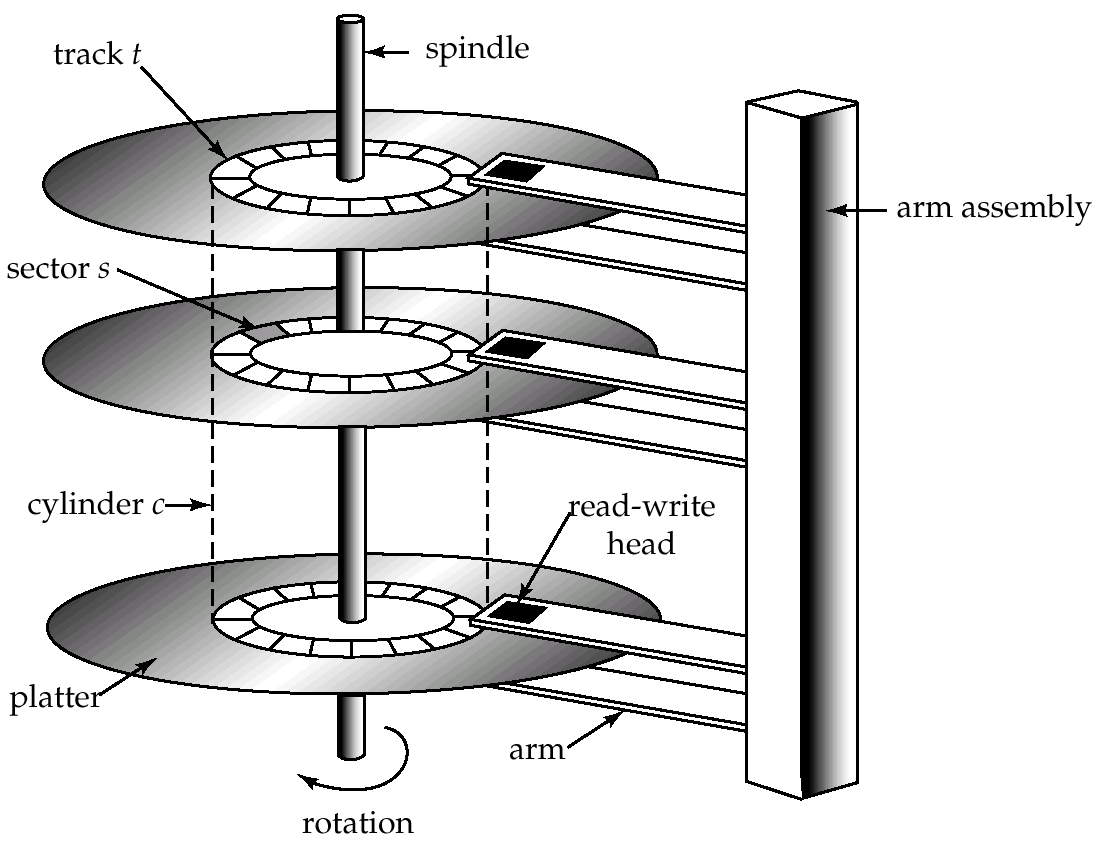
\includegraphics[width=.5\textwidth]{figure/磁盘.png}
    \caption{磁盘的物理结构}
\end{figure}

磁盘性能度量:
\begin{itemize}
    \item 访问时间
    \item 寻道时间(seek time): 平均寻道时间是最大寻道时间的1/3
    \item 旋转等待时间(rotational latency time): 平均旋转时间是旋转一周的1/2
    \item 数据传输率(data-transfer rate): 25$\sim$100兆/秒
\end{itemize}

磁盘访问优化:
\begin{itemize}
    \item 调度: 电梯算法
    \item 磁盘块的大小: 小, 更多的磁盘传输次数 vs. 大, 空间浪费
    \item 文件组织: 按与预期数据访问方式最接近的方式组织磁盘块 + 碎片整理
    \item 日志磁盘: 顺序写, 消除寻道时间 + 检查点
\end{itemize}

发掘磁盘顺序读的性能:
\begin{itemize}
    \item 预读(prefetch): 利用局部性原理.
\end{itemize}


\section{廉价磁盘冗余阵列(RAID)}

廉价磁盘冗余阵列: Redundant Arrays of Inexpensive Disks, RAID. 是一种利用大量廉价磁盘进行磁盘组织的技术.
\begin{itemize}
    \item 价格: 大量廉价的磁盘比少量昂贵的大磁盘合算得多
    \item 性能: 大量磁盘可以提高数据的并行存取
    \item 可靠性: 冗余数据可以存放在多个磁盘上, 单个磁盘的故障不会导致数据丢失
\end{itemize}
\begin{remark}
    过去RAID是大而昂贵的磁盘的替代方法, 今天使用RAID是因为它的高可靠性和高数据传输率. 因此``I''代表independent, 而非inexpensive.
\end{remark}

\begin{definition}[冗余(Redundancy)]
    冗余(Redundancy): 存储额外信息以便当磁盘故障时能从中重建.
\end{definition}

\begin{definition}[镜像冗余]
    \begin{itemize}
        \item 一个逻辑磁盘由两个物理磁盘组成, 写操作在每个磁盘上执行
        \item 如果其中一个发生故障, 数据可以从另一个磁盘读出
        \item 只有第一个磁盘故障尚未恢复, 第二个磁盘也发生故障, 这时才会发生数据丢失
    \end{itemize}
\end{definition}

\begin{definition}[校验码冗余]
    \textcolor{red}{纠错码(Error Correcting Code, ECC)}: 内存中每个字节都有一个奇偶校验位与之相连, 它记录该字节中为1的比特位的总数是偶数(=0)还是奇数(=1), 如果字节中有一位被破坏, 则字节的ECC与存储的ECC就不会相匹配; \textcolor{red}{通过ECC可以检测到所有的1位错误}.
\end{definition}

通过拆分提高并行:
\begin{itemize}
    \item 将数据拆分到多个磁盘上以提高传输率
    \item 通过并行提高性能的两种途径:
    \begin{itemize}
        \item 负载平衡多个小的存取操作(即页面存取), 以提高这种存取操作的吞吐量
        \item 并行执行大的存取操作, 以减少大的存取操作的响应时间
    \end{itemize}
    \item 两种不同的拆分方式:
    \begin{itemize}
        \item 比特级拆分(Bit-level striping): 将每个字节按比特分开, 存储到多个磁盘上. 对于由4个磁盘组成的阵列, 将每个字节的第$i$个比特位和第$i+4$个比特位写到第$i$个磁盘上, 其存取速度是单个磁盘的8倍.
        \item 块级拆分(Block-level striping): 对于由$n$个磁盘构成的阵列, 文件的第$i$块存放在第$(i \text{ mod } n) + 1$个磁盘上.
    \end{itemize}
\end{itemize}

\textcolor{red}{Hint: 下面介绍不同RAID级别. 比较重要的是RAID 1和RAID 5.}

\subsection{RAID 0}

RAID 0: 块级拆分且没有任何冗余的磁盘阵列, 用于高性能访问且数据丢失不十分重要的应用场合.

\subsection{RAID 1}

带块级拆分的磁盘镜像, 提供最佳写性能, 一般用于类似于数据库系统中日志文件存储的应用场合.
\begin{figure}[H]
    \centering
    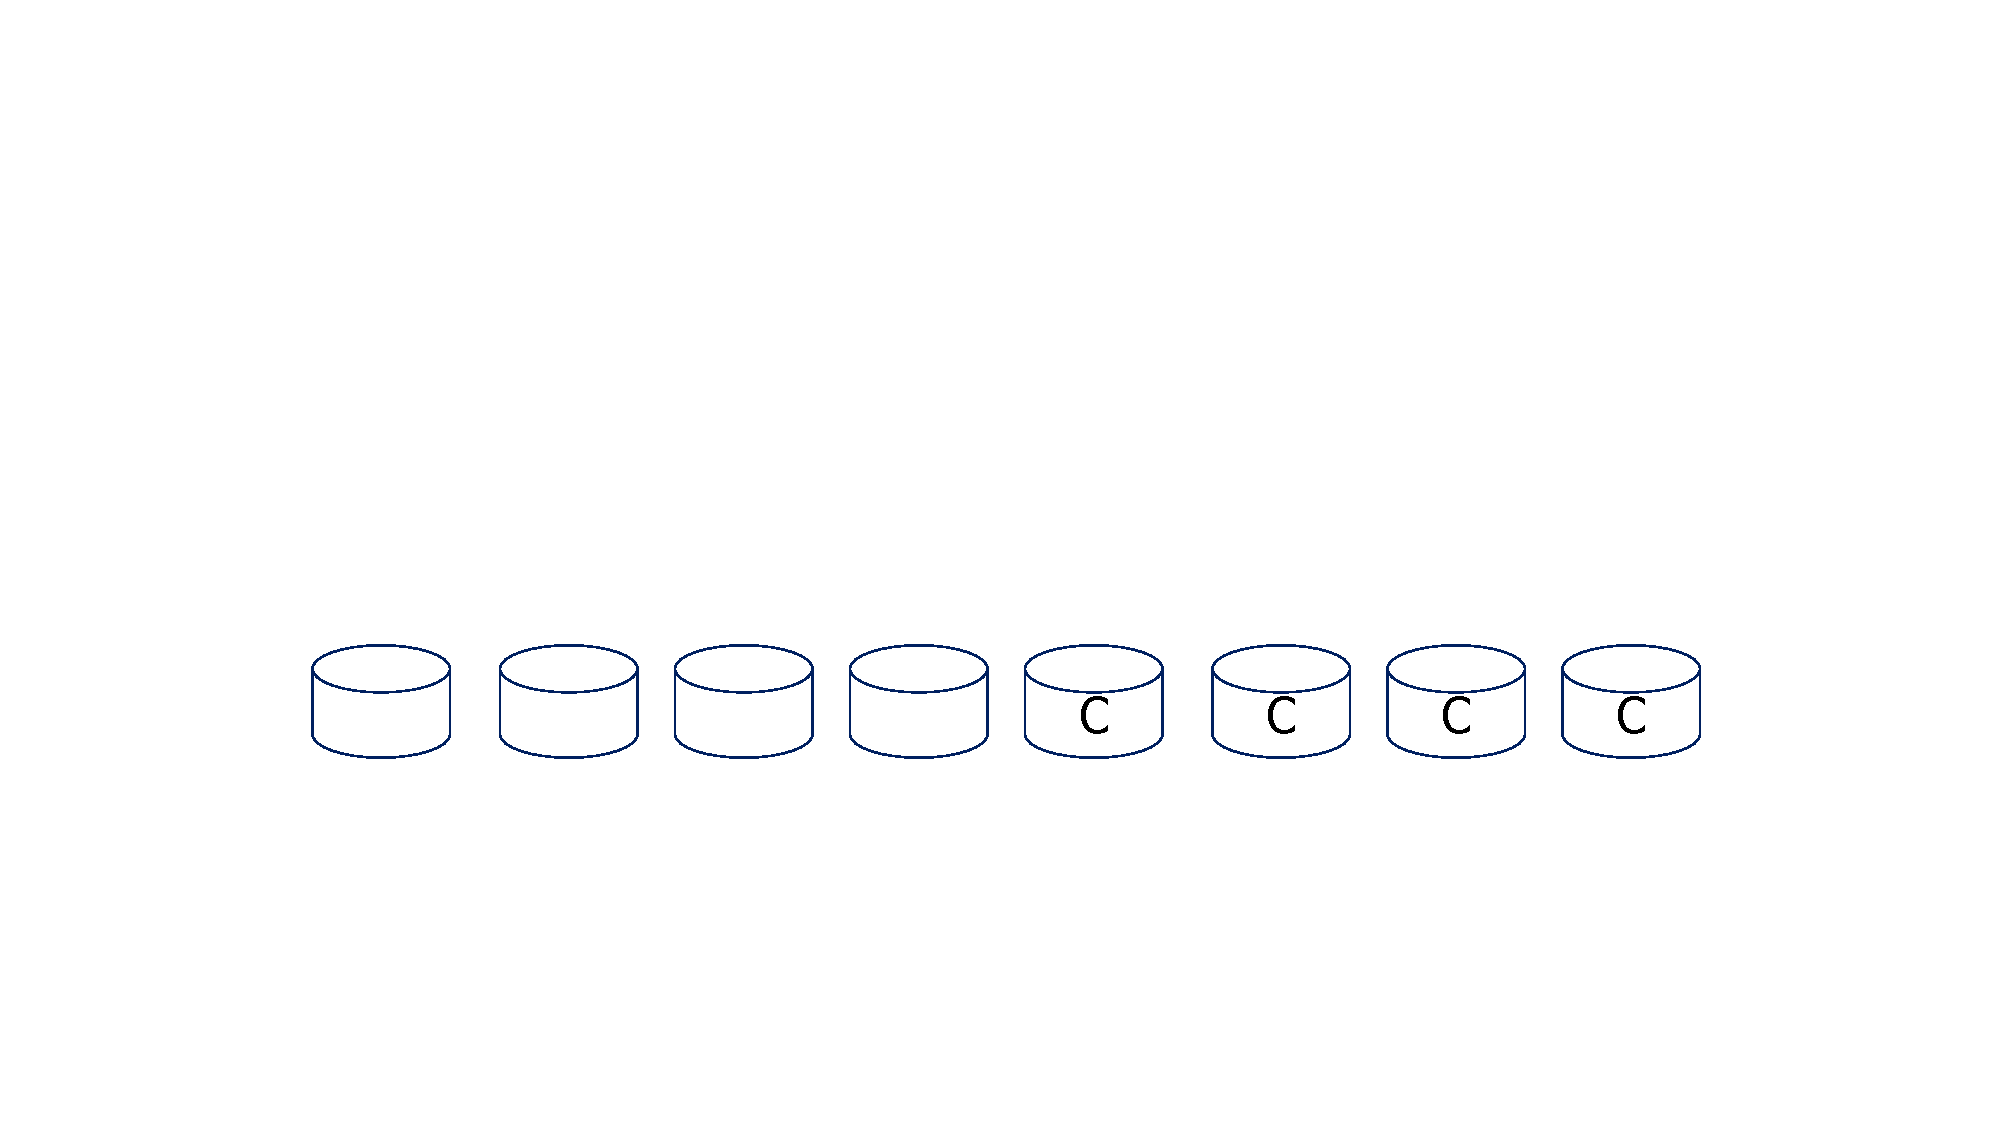
\includegraphics[width=.6\textwidth]{figure/RAID-1.pdf}
    \caption{RAID 1: 无冗余拆分}
\end{figure}

\subsection{RAID 3: 位交叉奇偶校验}

\begin{figure}[H]
    \centering
    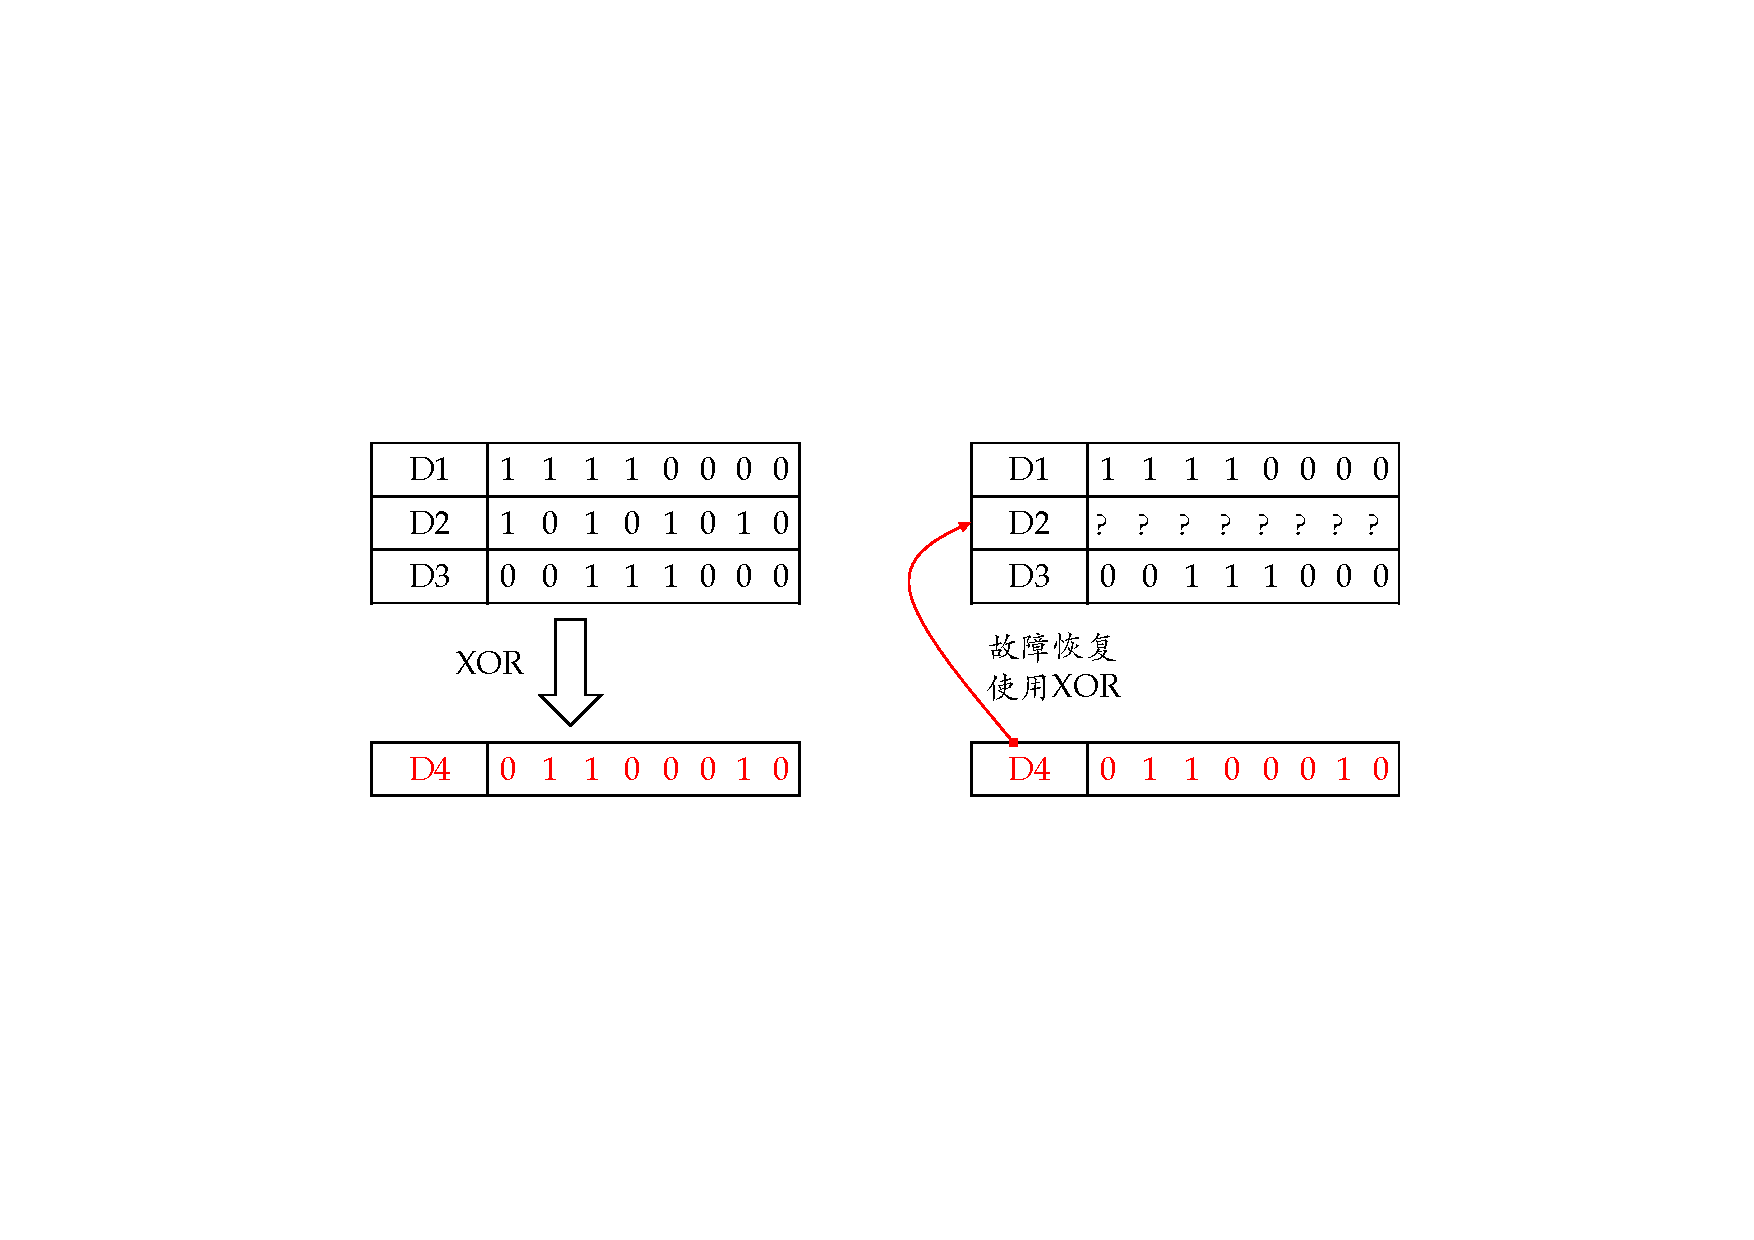
\includegraphics[width=.6\textwidth]{figure/RAID-3.pdf}
    \caption{RAID 3: 位交叉奇偶校验}
\end{figure}

奇偶校验值的计算是以各个硬盘的相对应位进行异或的逻辑运算, 然后将结果写入奇偶校验硬盘.

\subsection{RAID 4: 块交叉奇偶校验}

块级拆分, 在一个独立的磁盘上为其他$N$个磁盘上对应的块保留一个奇偶校验块.

读取一个块只访问一个磁盘, 每个存取操作的传输率低, 但可以并行地执行多个读操作, 从而产生较高的总I/O率.

\subsection{RAID 5: 块交叉的分布奇偶校验}

将数据和奇偶校验位分布到所有的$N$个磁盘上.
\begin{itemize}
    \item 奇偶校验块不能和这个块对应的数据存储在同一个磁盘上 $\to$ 一个磁盘坏了就可以立刻重建其数据;
    \item RAID 5所有磁盘都参与对读请求的服务, 而RAID 4中奇偶校验磁盘不参与读操作;
    \item RAID 5包容RAID 4, 在相同成本下提供更好的读写性能.
\end{itemize}

\begin{figure}[H]
    \centering
    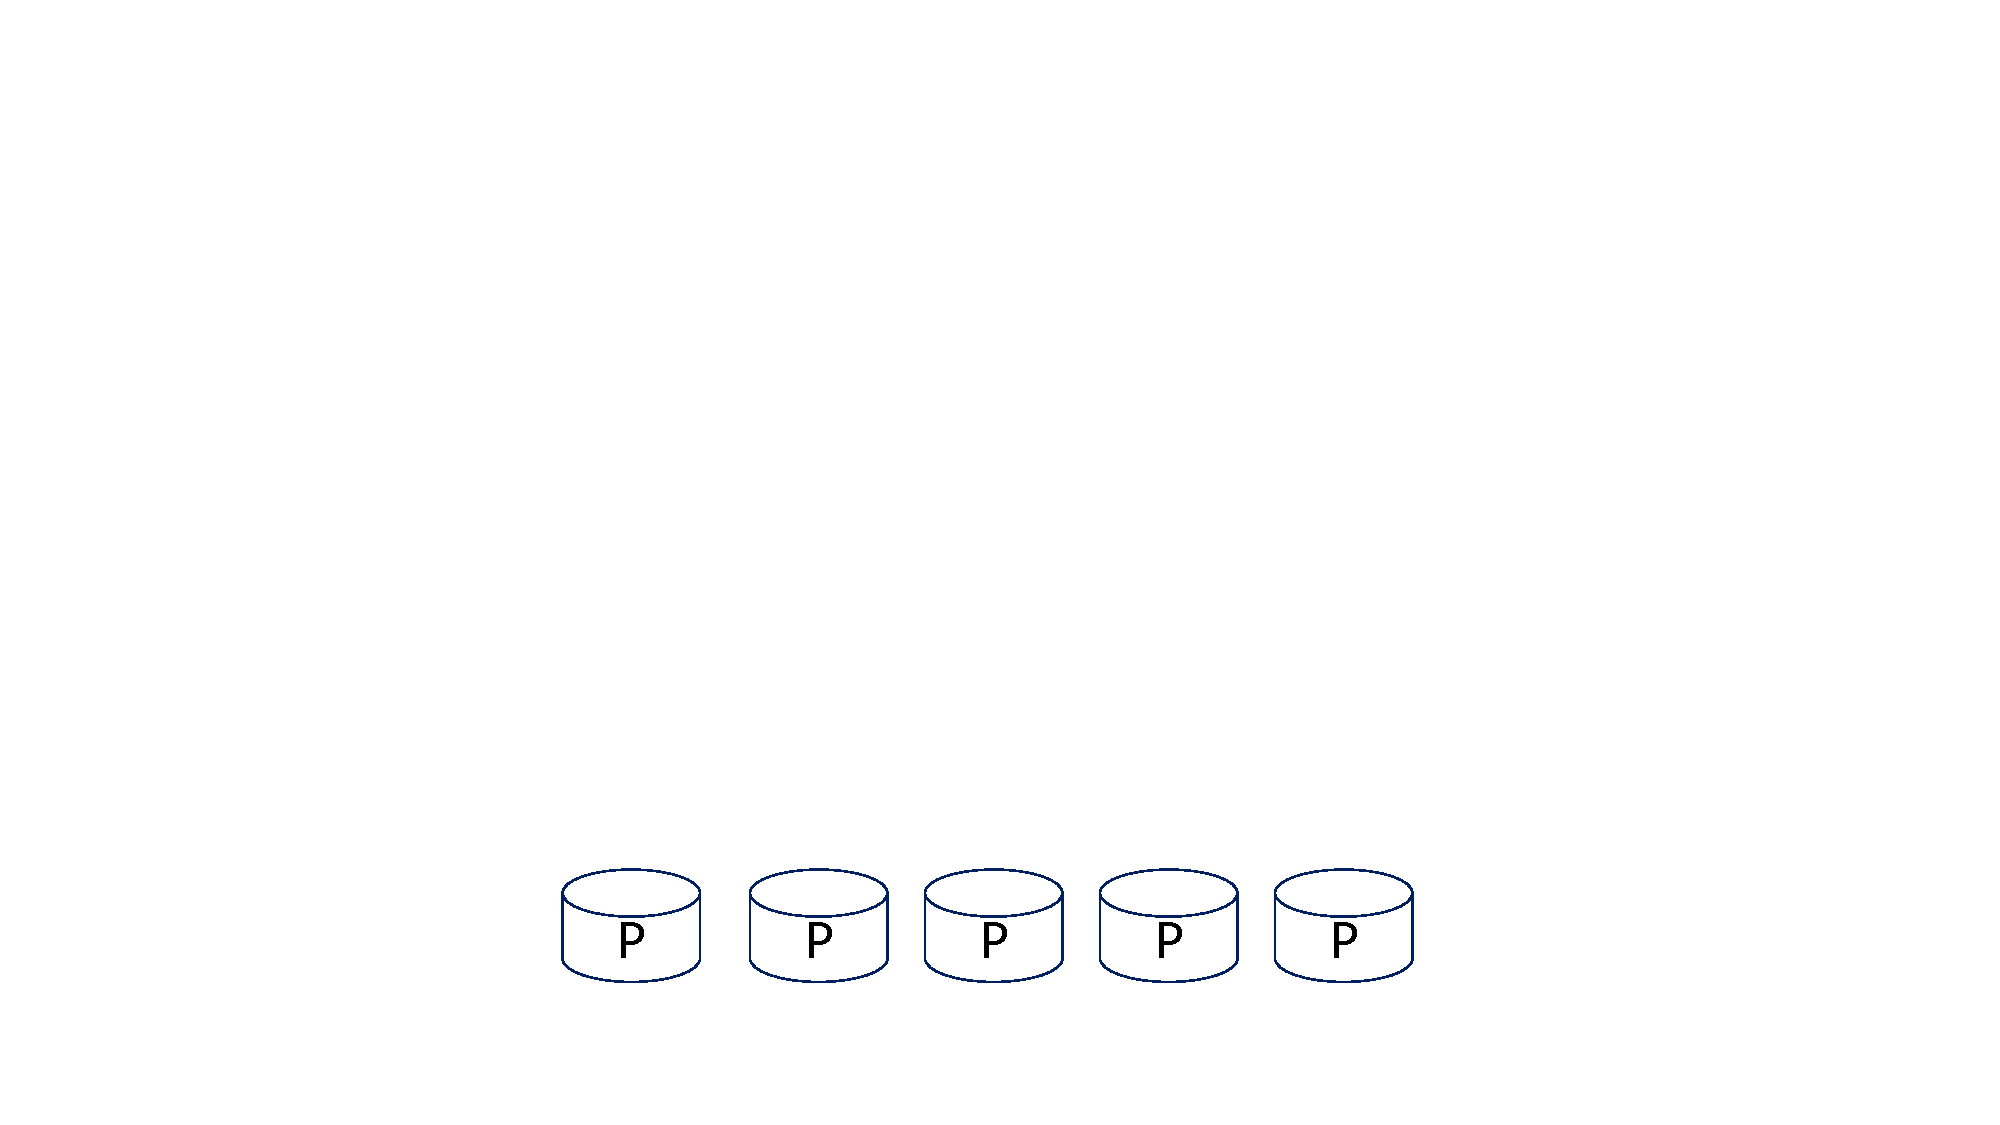
\includegraphics[width=.4\textwidth]{figure/RAID-5.pdf}
    \caption{RAID 5: 块交叉的分布奇偶校验}
\end{figure}

\subsection{RAID 6}

反正很可靠就对了.

\subsection{RAID总结}

\begin{itemize}
    \item RAID 0: 高性能, 可靠性差.
    \item RAID 1: 最佳写性能, 开销大.
    \item RAID 3: 高数据传输率, 大数据量.
    \item RAID 5: 高的总I/O率, 适合随机读, 大数据量.
    \item RAID 6: 高可靠性.
\end{itemize}

\subsection{选择合适的RAID级别}

如果应用需要每秒$r$次读, $w$次写:
\begin{itemize}
    \item RAID 1 要求每秒$r+2w$次I/O操作;
    \item RAID 5 要求每秒$r+4w$次I/O操作; 
    
    一次写操作实际上涉及到4次I/O操作: 读取旧数据、读取旧奇偶校验、写入新数据、写入新奇偶校验.
    \item RAID 5 比 RAID 1 使用较少的磁盘可能是幻觉. \textit{比如说需要1TB, 每个磁盘是1TB. 使用RAID 1需要2块磁盘, 使用RAID 5需要至少3块磁盘. (如果只有两块磁盘, 那谁和谁进行异或呢?)}
\end{itemize}

\textcolor{red}{当写操作较少且数据非常大时, RAID 5较优, 否则RAID 1更佳.}

\textbf{RAID的Write Back}: RAID控制器先把数据放入自身缓存, 后续再写入.

\section{缓冲区}

为快速找到页面, 内存页面地址被散列dbid-fileno-pageno标识(数据库ID, 文件号、页面号)的hash地址.

当需要访问一个磁盘块时:
\begin{itemize}
    \item 如果该块已在缓冲区中, 返回块在内存中的地址;
    \item 如果块不在缓冲区中,
    \begin{itemize}
        \item 缓冲区管理器为该块在缓冲区中分配空间, 如果有必要, 替换缓冲区中的其他块
        \item 如果被替换的块被修改过, 则将其写回磁盘
        \item 将所需块调入缓冲区, 返回其在缓冲区的地址
    \end{itemize}
\end{itemize}

缓冲区管理中的特殊内存块:
\begin{itemize}
    \item 被钉住的块(pinned blocks): 不允许写回磁盘的块.
    \begin{itemize}
        \item 当一个块上的更新正在进行时, 不允许写回磁盘
        \item 可以钉住被频繁访问的小表
    \end{itemize}
    \item 块的强制刷出(forced output of blocks):
    \begin{itemize}
        \item 先写日志原则: 被更新的数据页刷出时, 对应的日志记录被强制刷出
        \item 生成检查点时, 日志和数据缓冲区被强制刷出
        \item 提交事务时, 其日志记录被强制刷出
    \end{itemize}
\end{itemize}


\textbf{替换策略}:
\begin{itemize}
    \item LRU
    \item MRU(最近最常使用): e.g., 在进行连接$R \bowtie S$时, $R$中的一个元组一旦被处理完就不再需要了, 同时$S$中的一个元组要等待其他元组做完, 这个时候就应该使用MRU.
\end{itemize}

SQL Server缓冲区管理: Lazywriter(缓冲池管理器), 使用时钟算法.

...

多大缓冲区是合适的?
\begin{itemize}
    \item 若一个页面每秒被访问$n$次, 将它驻留在内存节省
    \begin{align*}
        n \times \frac{\text{price-per-disk-drive}}{\text{accesses-per-second-per-disk}}
    \end{align*}
    \item 保持一个页面在内存的代价
    \begin{align*}
        \frac{\text{price-per-MB-of-memory}}{\text{pages-per-MB-of-memory}}
    \end{align*}
    \item 5-minute rule: 如果一个被随机访问的页面的使用频率超过每5分钟一次, 那么它应该被驻留在内存
    \item 1-minute rule: 如果一个被随机访问的页面的使用频率超过每1分钟一次, 那么它应该被驻留在内存
\end{itemize}


\section{数据库存储结构}

\begin{figure}[H]
    \centering
    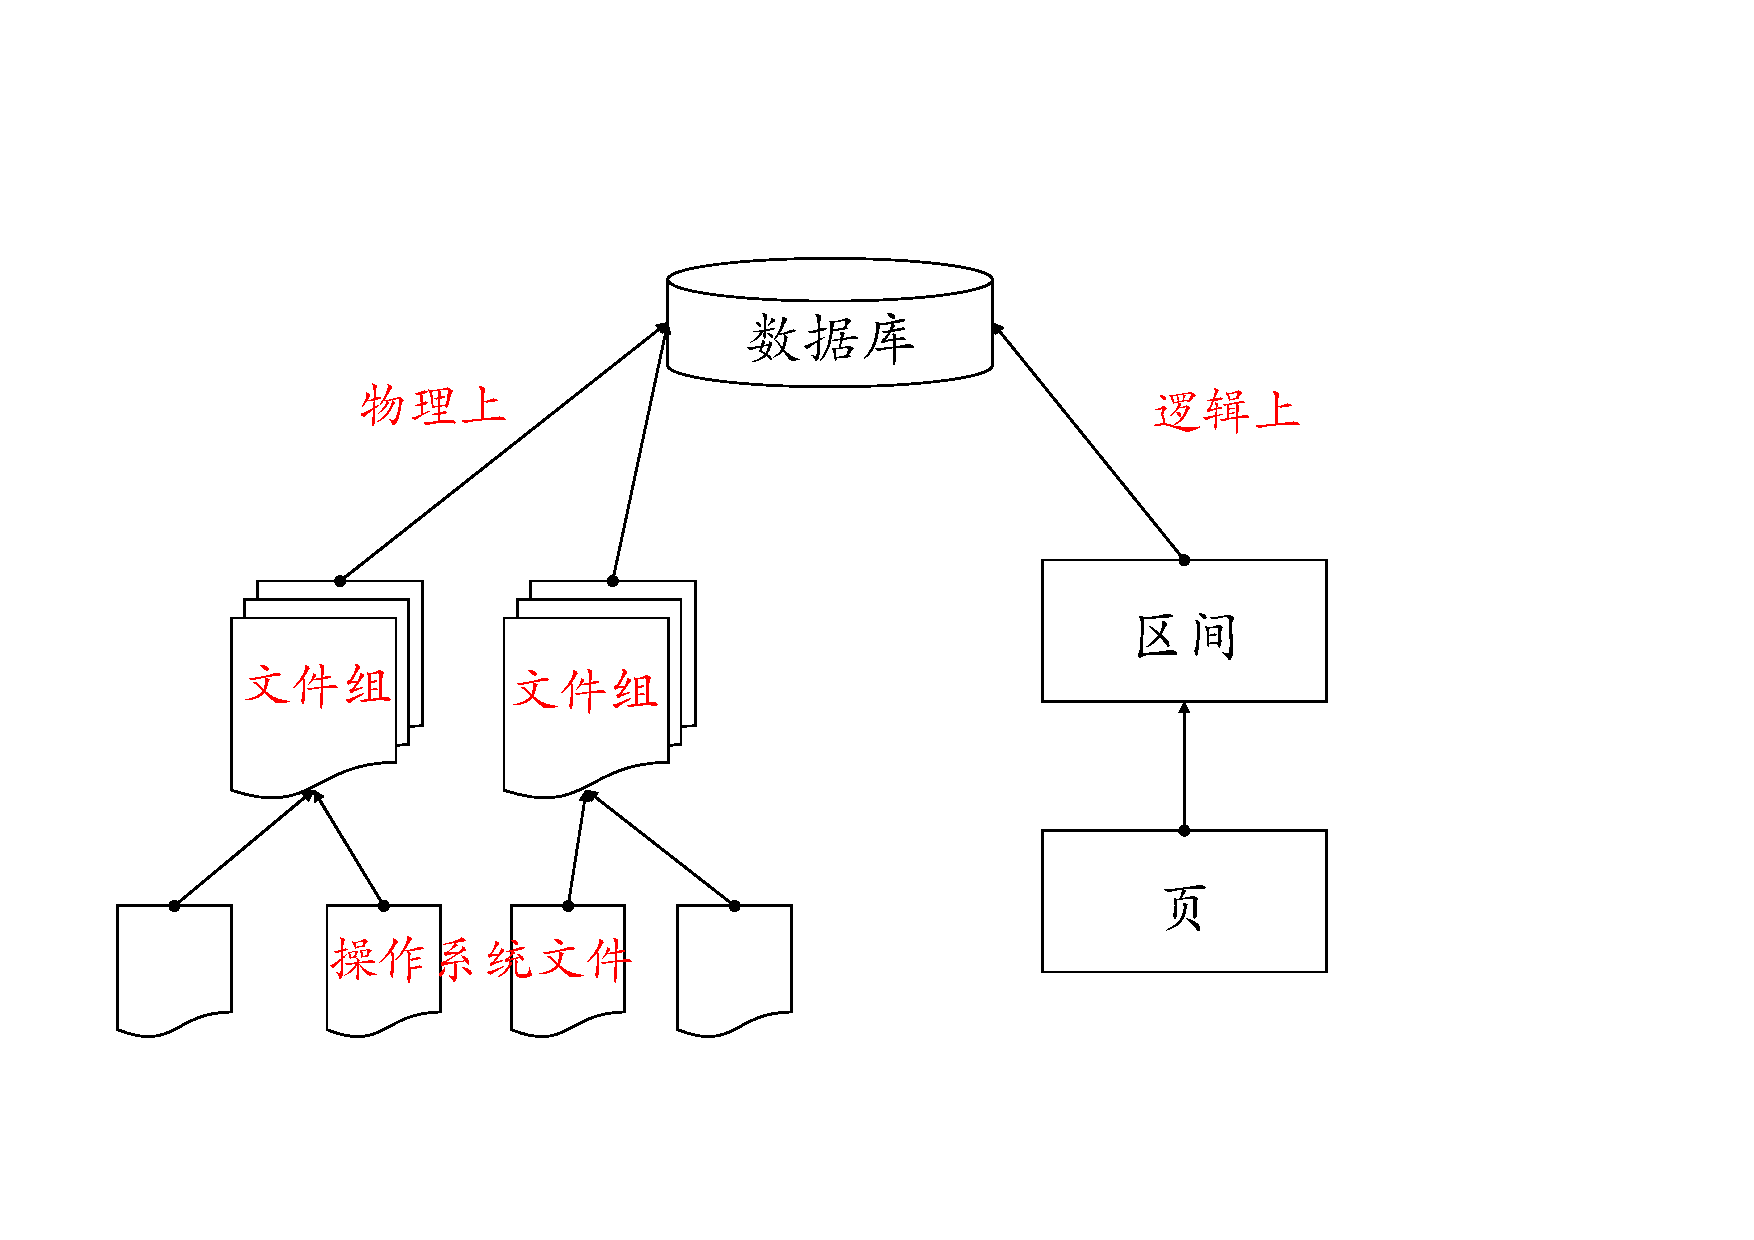
\includegraphics[width=.6\textwidth]{figure/数据库结构.pdf}
    \caption{数据库存储结构}
\end{figure}

\subsection{页面与区间}

\begin{itemize}
    \item 数据文件被划分成8k的页面;
    \item 每个文件中的页面号都以0开始;
    \item 页面号的形式为(file\#:page\#), 如(3:124);
    \item 8个连续页面构成一个区间——64k, 总是从能被8整除的页面开始;
    \item 存储分配总是按照区间为单位进行, 对象每次增长1个区间;
    \item I/O可以按页面(8 KB)或者区间(64 KB)来进行.
\end{itemize}

如何为对象分配空间?
\begin{itemize}
    \item GAM
    \item PFS
\end{itemize}

如何找到对象占据的空间?
\begin{itemize}
    \item IAM
\end{itemize}

行在页内是如何存储的?

\subsection{GAM - 全局分配位图(bitmap)}

\begin{itemize}
    \item 记录文件当中哪些区间已经被分配的页面, 可以看成是一个8000个字节的位图, 每个位代表一个区间;
    \item 位0代表区间0, 位1代表区间8, 位2代表区间16
    \item 0: 被使用; 1: 未使用;
    \item 差不多64000位, 所以可以表示64000个区间;
    \item 表达4GB数据空间, 如果文件大于4GB, 增加新的GAM页.
\end{itemize}

\subsection{PFS - 空闲页空间}

\begin{itemize}
    \item 记录文件中每个页面是否已经被分配以及有多少空闲空间;
    \item 每一个页面在PFS页中有一个字节对应
    \item 每个PFS覆盖8088个连续页面(64 MB)
    \item 页面充满度: 0, 1-50\%, 51-80\%, 81-95\%, 96-100\%
    \item 第一个PFS位于文件的第二个页面(page1), 以后每8088都是一个PSF页
\end{itemize}

\subsection{IAM - 索引分配位图}

如何发现一个特定对象的区间或页面?
\begin{itemize}
    \item 每个表/索引都至少有一个IAM, 记录该对象拥有哪些区间;
    \item IAM覆盖的范围与GAM相同, 如果位为1, 说明该区间被分配给该对象, 如果位为0, 说明该区间未被分配给该对象;
    \item 如11000000, 说明第一、二个区间被分配给该对象;
    \item 一个对象每占据文件的4G空间, 就需要一个IAM, 对象的所有IAM构成一个双向链表.
\end{itemize}

\subsection{基本页结构}

所有页面包括\textcolor{red}{页面头、页面体、页面槽}.

\begin{figure}[H]
    \centering
    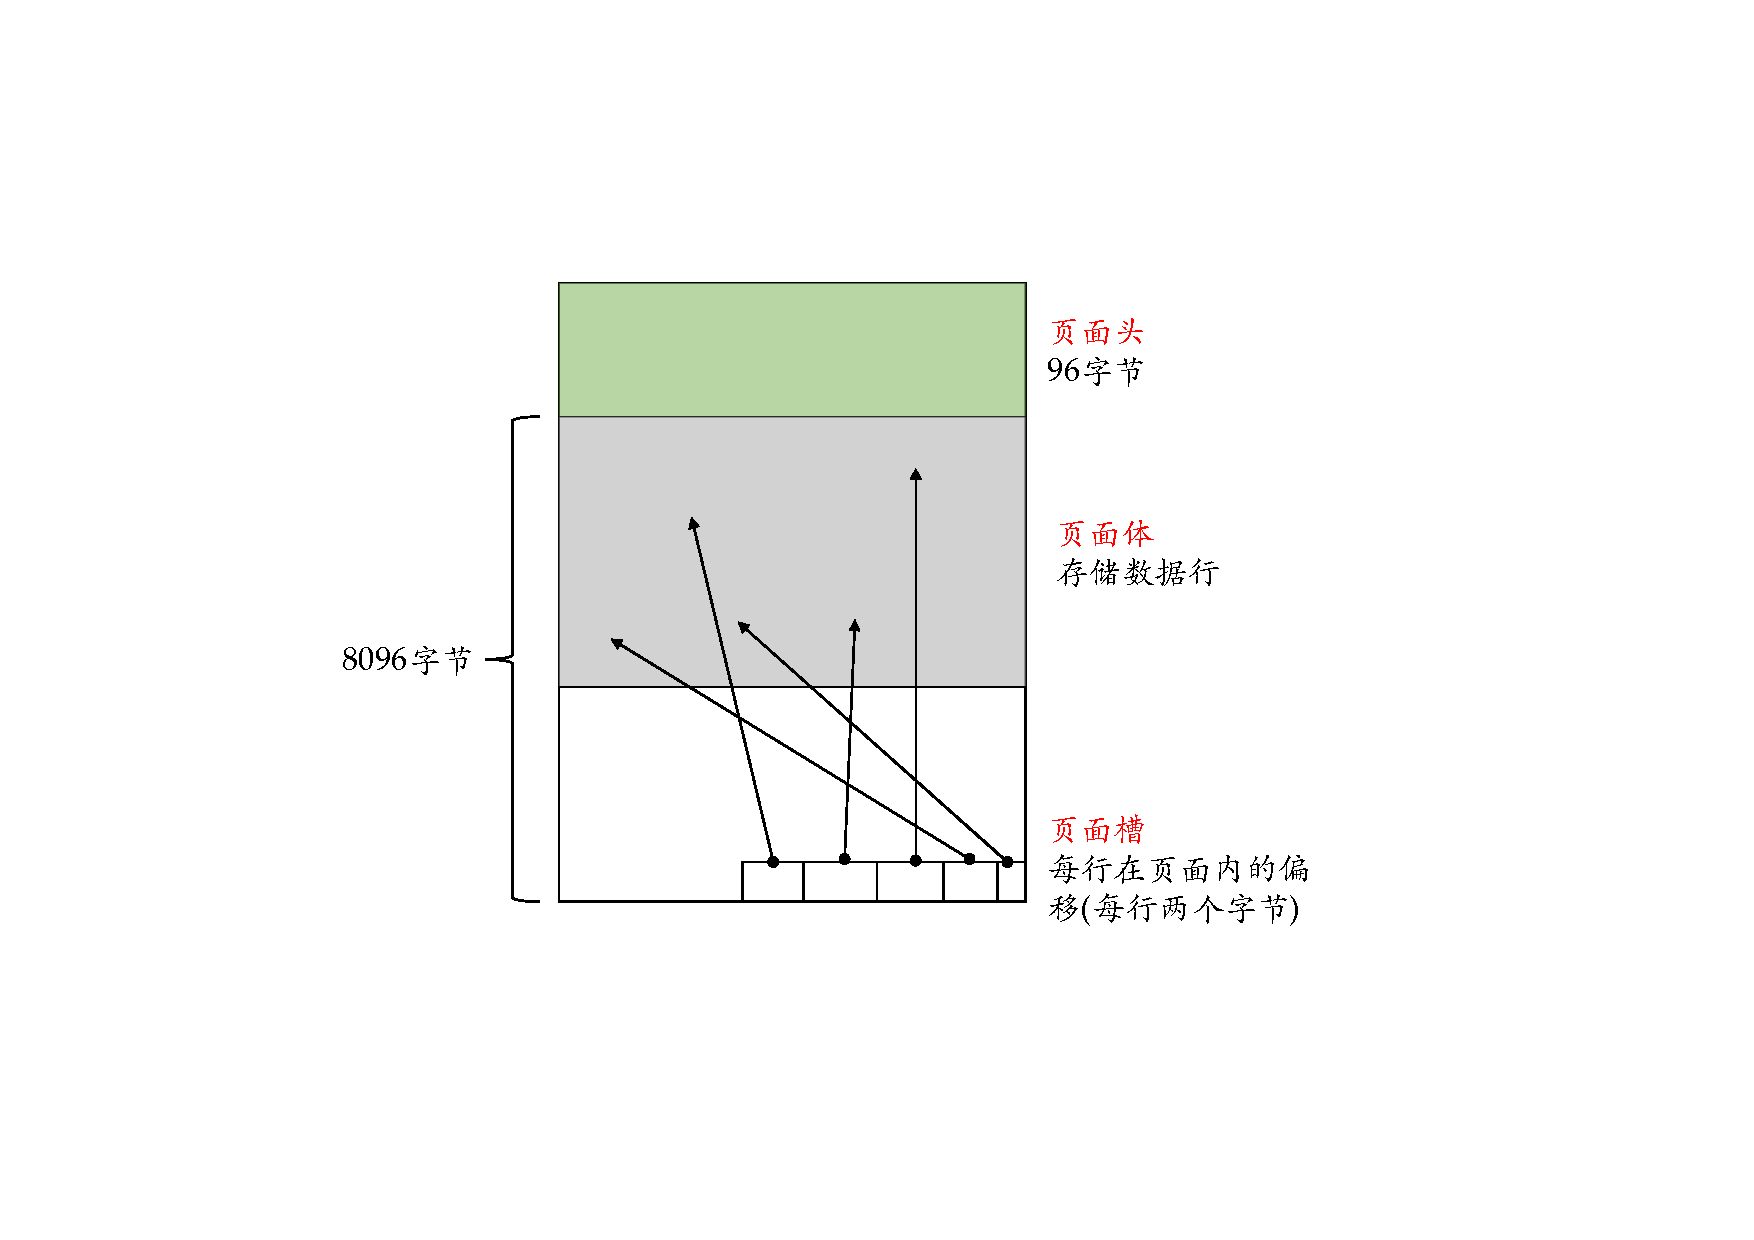
\includegraphics[width=.6\textwidth]{figure/基本页结构.pdf}
    \caption{基本页结构}
\end{figure}

\textbf{页头字段含义}:

\begin{longtable}{|p{3cm}|p{10cm}|}
\hline
\textbf{Field} & \textbf{What It Contains} \\
\hline
\endfirsthead

\hline
\textbf{Field} & \textbf{What It Contains} \\
\hline
\endhead

pageID & 数据库中该页的文件号和页号 \\
\hline
nextPage & 在页链中该页的下一页的文件号和页号 \\
\hline
prevPage & 在页链中该页的上一页的文件号和页号 \\
\hline
objID & 该页所属对象的ID \\
\hline
lsn & 用于修改该页的日志序列号(LSN) \\
\hline
slotCnt & 该页上槽的总数 \\
\hline
level & 该页在索引中的级别(对于叶级别该值为0) \\
\hline
indexId & 该页的索引ID(对于数据页该值为0) \\
\hline
freeData & 该页第一个空闲空间的字节偏移量 \\
\hline
pminlen & 行的固定长度部分的字节数 \\
\hline
freeCnt & 该页上空闲字节的数目 \\
\hline
reservedCnt & 由所有事务保留的字节数 \\
\hline
xactreserved & 由最近启动的事务保留的字节数 \\
\hline
tornBits & 每个扇区1位,用于监测页分裂的写 \\
\hline
flagBits & 一个两字节的位置,包含有关该页的额外信息 \\
\hline

\end{longtable}

\textbf{数据行结构}:
\begin{figure}[H]
    \centering
    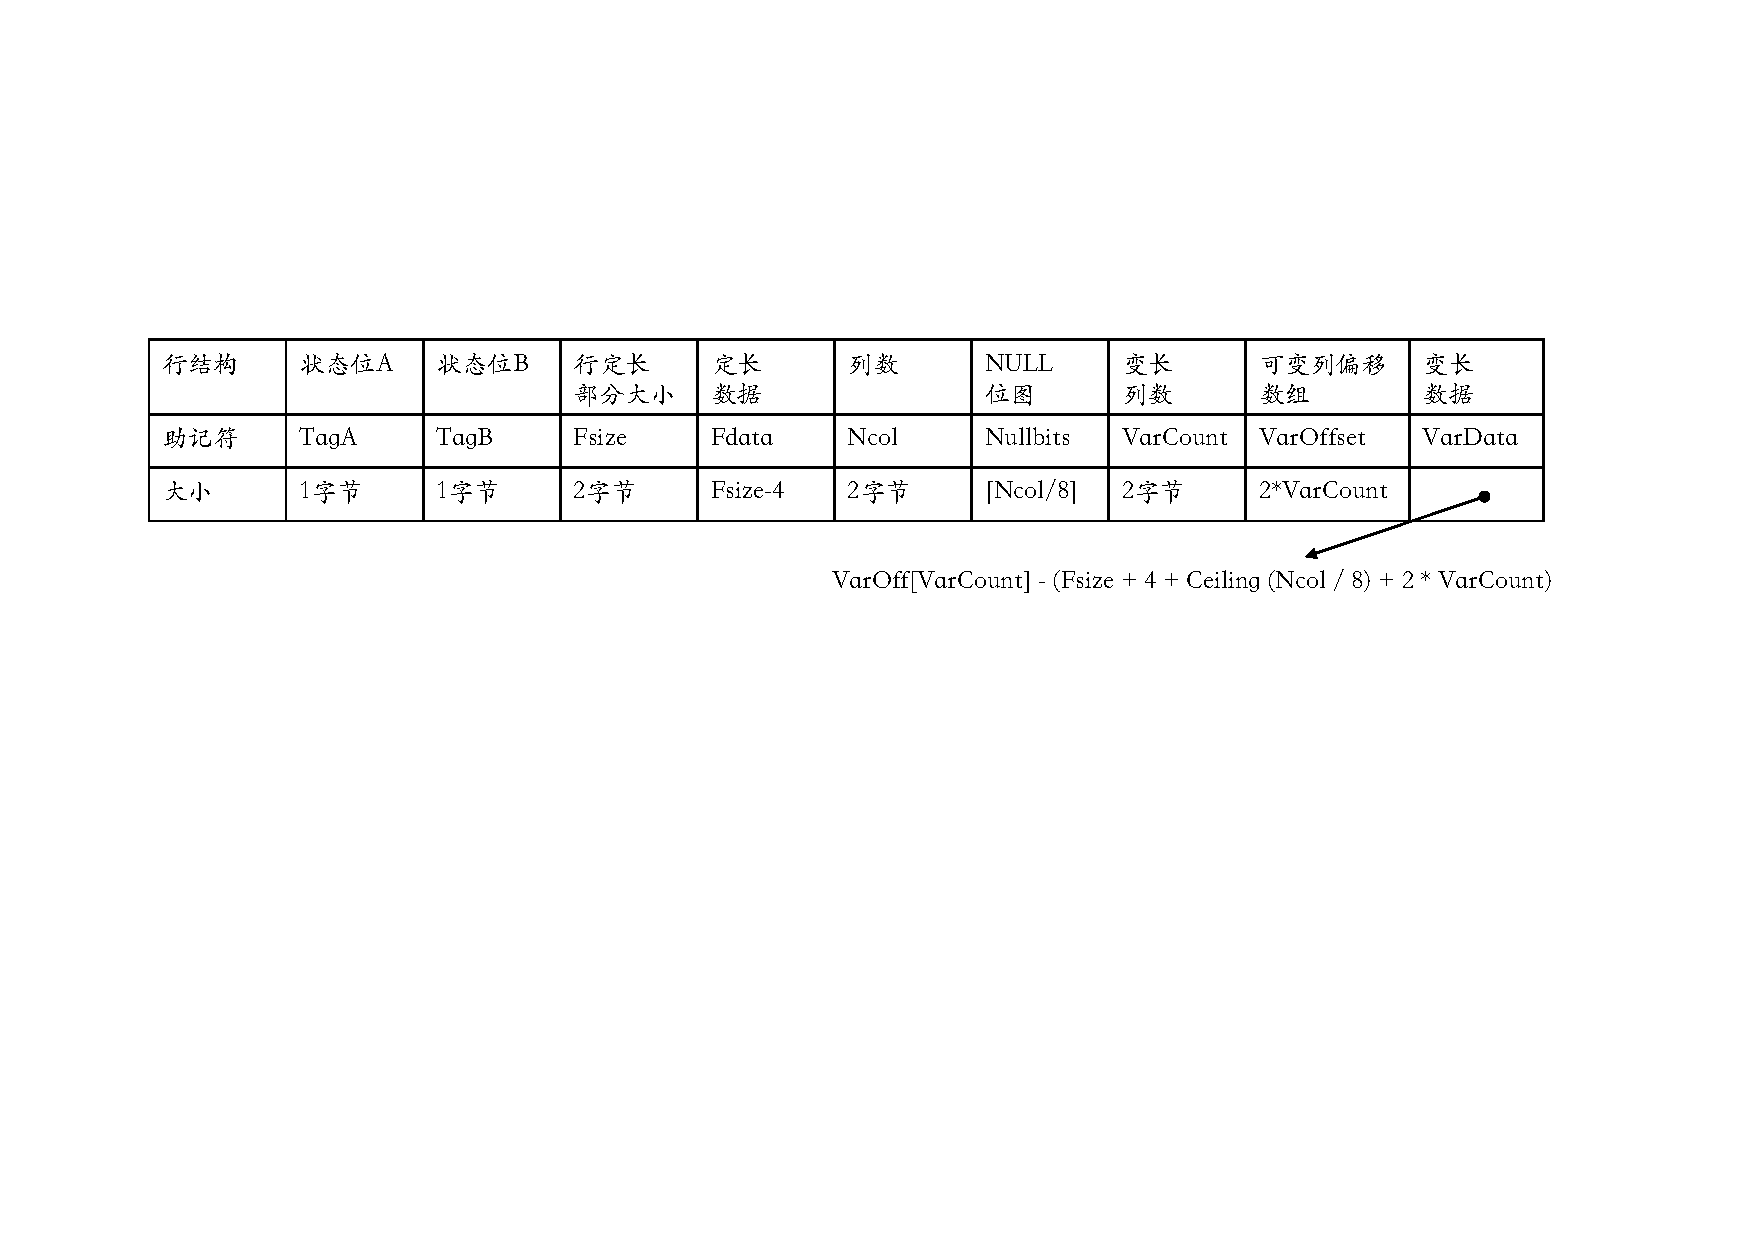
\includegraphics[width=1.1\textwidth]{figure/数据行结构.pdf}
    \caption{数据行结构}
\end{figure}

\section{索引}

\subsection{B+树索引}

我们首先来看叶节点:
\begin{figure}[H]
    \centering
    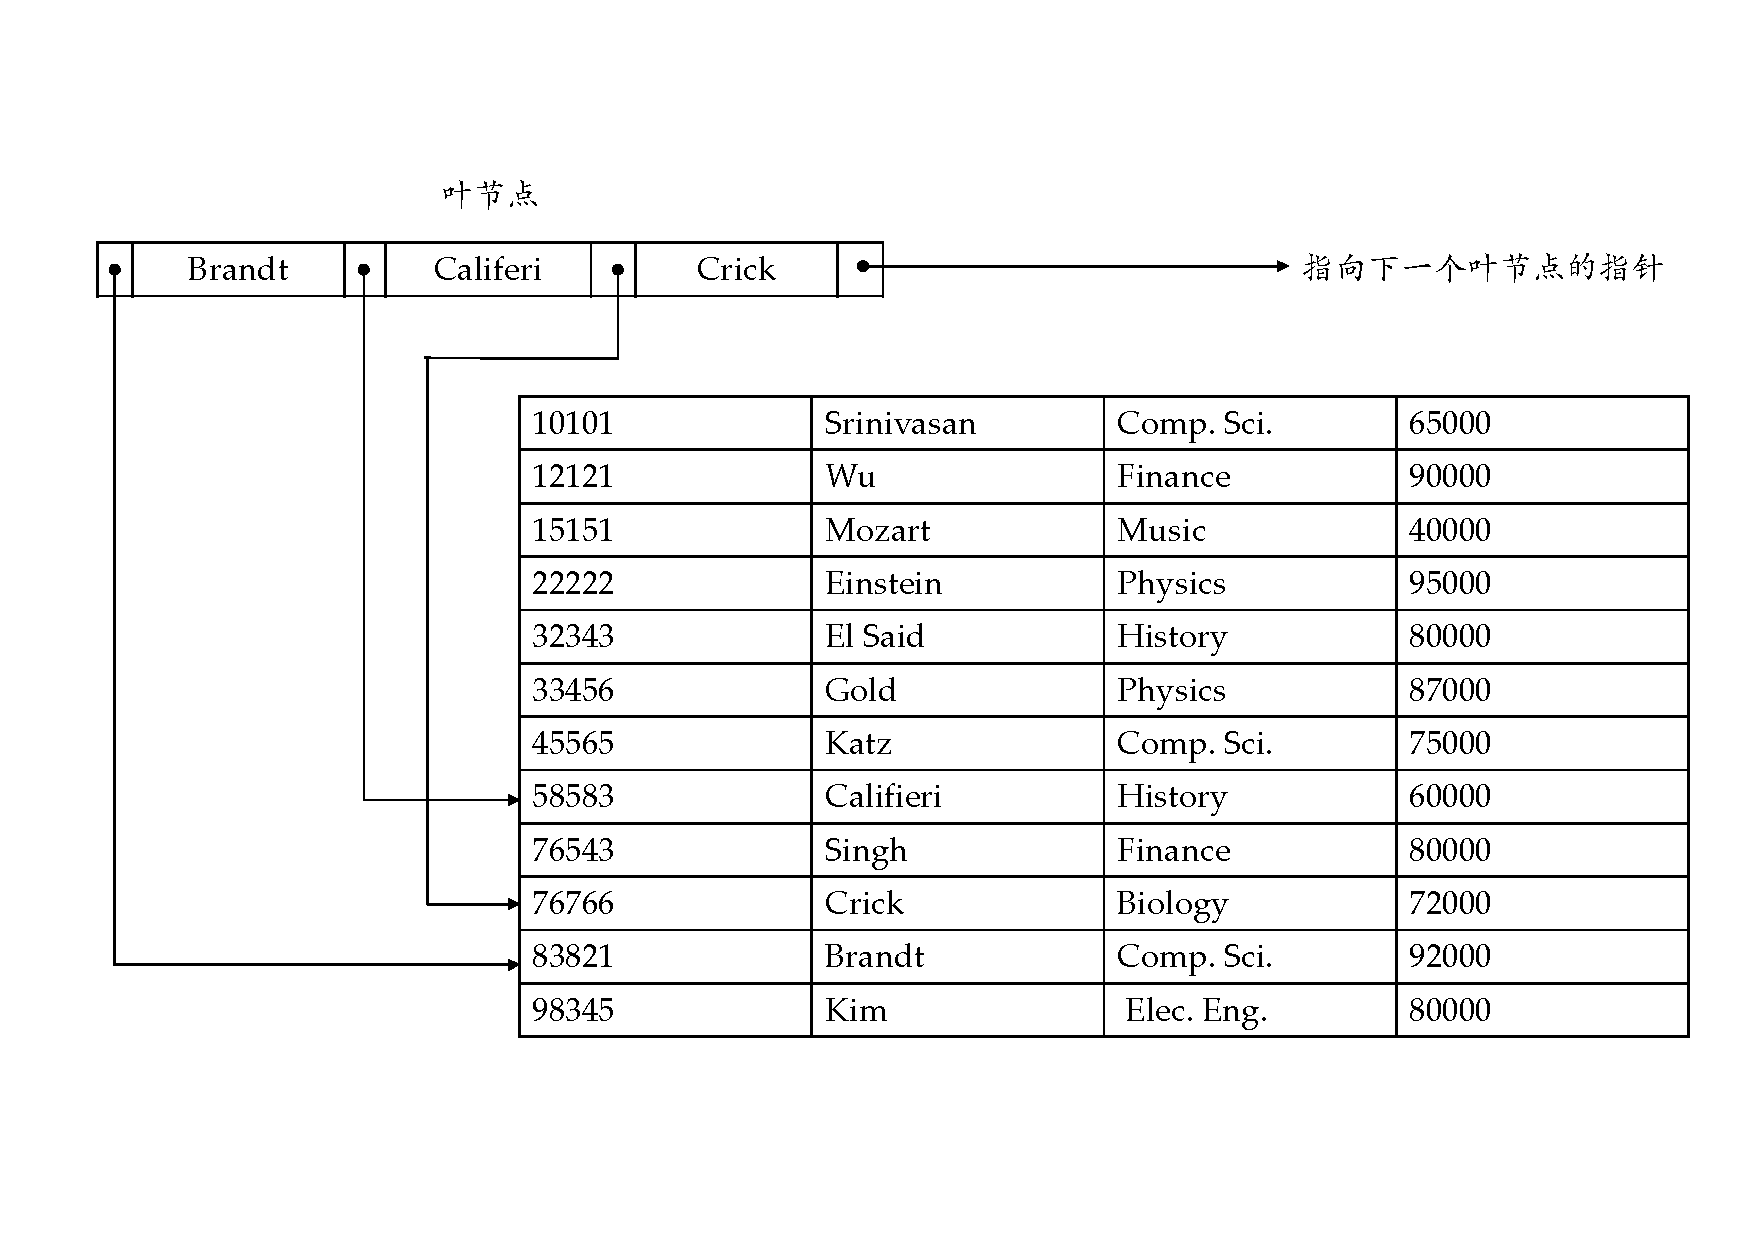
\includegraphics[width=.8\textwidth]{figure/B+叶节点.pdf}
    \caption{B+树的叶节点}
\end{figure}


如果此B+树的阶数是$m$, 则除了根之外的每个节点都包含最少$\lfloor m/2\rfloor$个元素最多 
$m-1$个元素, 对于任意的结点有最多$m$个子指针. 对于所有内部节点, 子指针的数目总是比元素的数目多一个. 所有叶子都在相同的高度上, 叶结点本身按关键字大小从小到大链接.

除了根之外每个非叶子节点有$\lceil n/2 \rceil \sim n$个子女. 有$n$个子女则含有$n-1$个码.
\begin{figure}[H]
    \centering
    \includegraphics[width=\textwidth]{figure/B+树.pdf}
    \caption{$n=4$的时候的B+树}
\end{figure}

在查找时, 若非叶子节点上的关键字等于给定值, 并不终止, 而是继续向下直到叶子节点. 
因此, 在 B+ 树中, 不管查找成功与否, 每次查找都是走了一条从根到叶子节点的路径.


\textbf{B+ 树的插入算法}:
\begin{enumerate}
    \item 若为空树, 创建一个叶子节点, 然后将记录插入其中, 此时这个叶子节点也是根节点, 插入操作结束.
    \item 根据关键字找到叶子节点, 向这个叶子节点插入记录. 插入后, 若当前节点关键字的个数小于$m$, 则插入结束. 否则将这个叶子节点分裂成左右两个叶子节点, 左叶子节点包含前$m/2$个记录, 右节点包含剩下的记录, 将第$m/2+1$个记录的关键字进位到父节点中(父节点一定是索引类型节点), 进位到父节点的关键字左孩子指针向左节点, 右孩子指针向右节点. 将当前节点的指针指向父节点, 然后执行第 3 步.
    \item 针对索引类型节点(内部节点): 若当前节点关键字的个数小于等于$m-1$, 则插入结束, 否则, 将这个索引类型节点分裂成两个索引节点, 左索引节点包含前$ (m-1)/2 $个key, 右节点包含$ m-(m-1)/2 $个 key, 将第 $m/2$个关键字进位到父节点中, 进位到父节点的关键字左孩子指向左节点, 进位到父节点的关键字右孩子指向右节点. 将当前节点的指针指向父节点, 然后重复这一步.
\end{enumerate}

\textbf{B+ 树的删除算法}:
\begin{enumerate}
    \item 首先查询到键值所在的叶子节点, 删除该叶子节点的数据.
    \item 如果删除叶子节点之后的数据数量, 满足: 关键字的个数大于等于$\lceil m/2 \rceil$, 则直接返回.
    \item 否则, 就需要做平衡操作: 如果该叶子节点的左右兄弟节点的数据量可以借用(选择多的那个), 就借用过来满足平衡条件. 否则, 就与相邻的兄弟节点合并成一个新的子节点了.
\end{enumerate}

B+树矮而胖: 假定树结点大小与磁盘块大小相等, 为4k, $n=100$, 有1百万个
搜索码, $\log_{50}(1 000 000)= 4$, 访问4个磁盘结点.

二叉树瘦而高.


InnoDB一颗B+树可以放多少行?
\begin{example}
    假定一个页16K, 一行1K, 一页存放16行.

    假定主码为bigint, 长度8字节, 指针6字节, 共14字节. 一个页中能存放16384/14=1170.

    一棵高度为2的B+树, 能存放1170*16=18720条这样的记录.

    一棵高度为2的B+树, 能存放1170*1170*16=21902400条这样的记录.
\end{example}

\subsection{散列索引}

\begin{itemize}
    \item 桶(bucket): 存储一条或多条记录的存储单元
    \item 散列(hash): 散列函数$h(K)=B$, $K$是搜索码, $B$是桶地址
    \begin{itemize}
        \item 分布是均匀的, 桶包含记录的个数是均匀的
        \item 分布是随机的, 散列值不能与搜索码值呈现出相关性
    \end{itemize}
    \item 桶溢出(bucket overflow): 因桶不足(insufficient bucket)或偏斜(skew)所致
\end{itemize}



\begin{figure}[H]
    \centering
    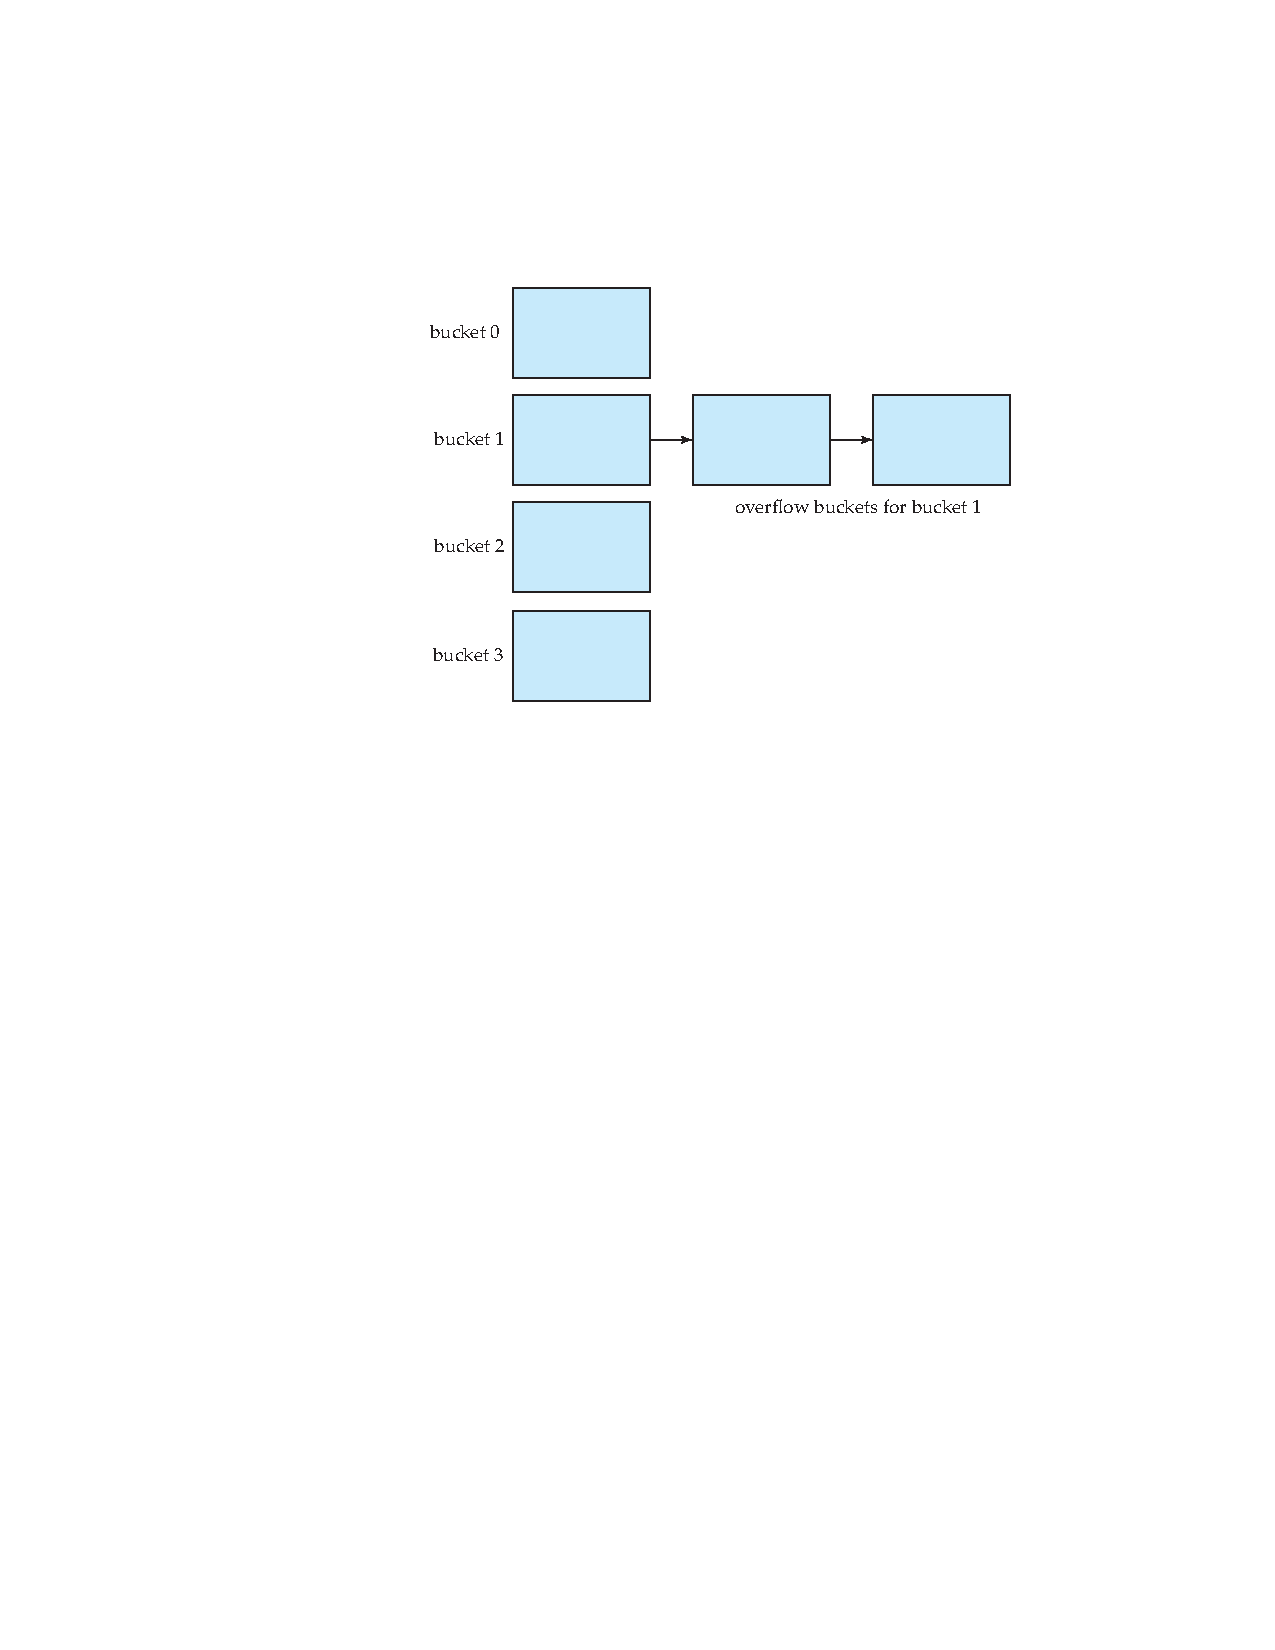
\includegraphics[width=.47\textwidth]{figure/溢出链.pdf}
    \caption{溢出链}
\end{figure}

桶溢出的时候, 在后面加上一条链.

\begin{figure}[H]
    \centering
    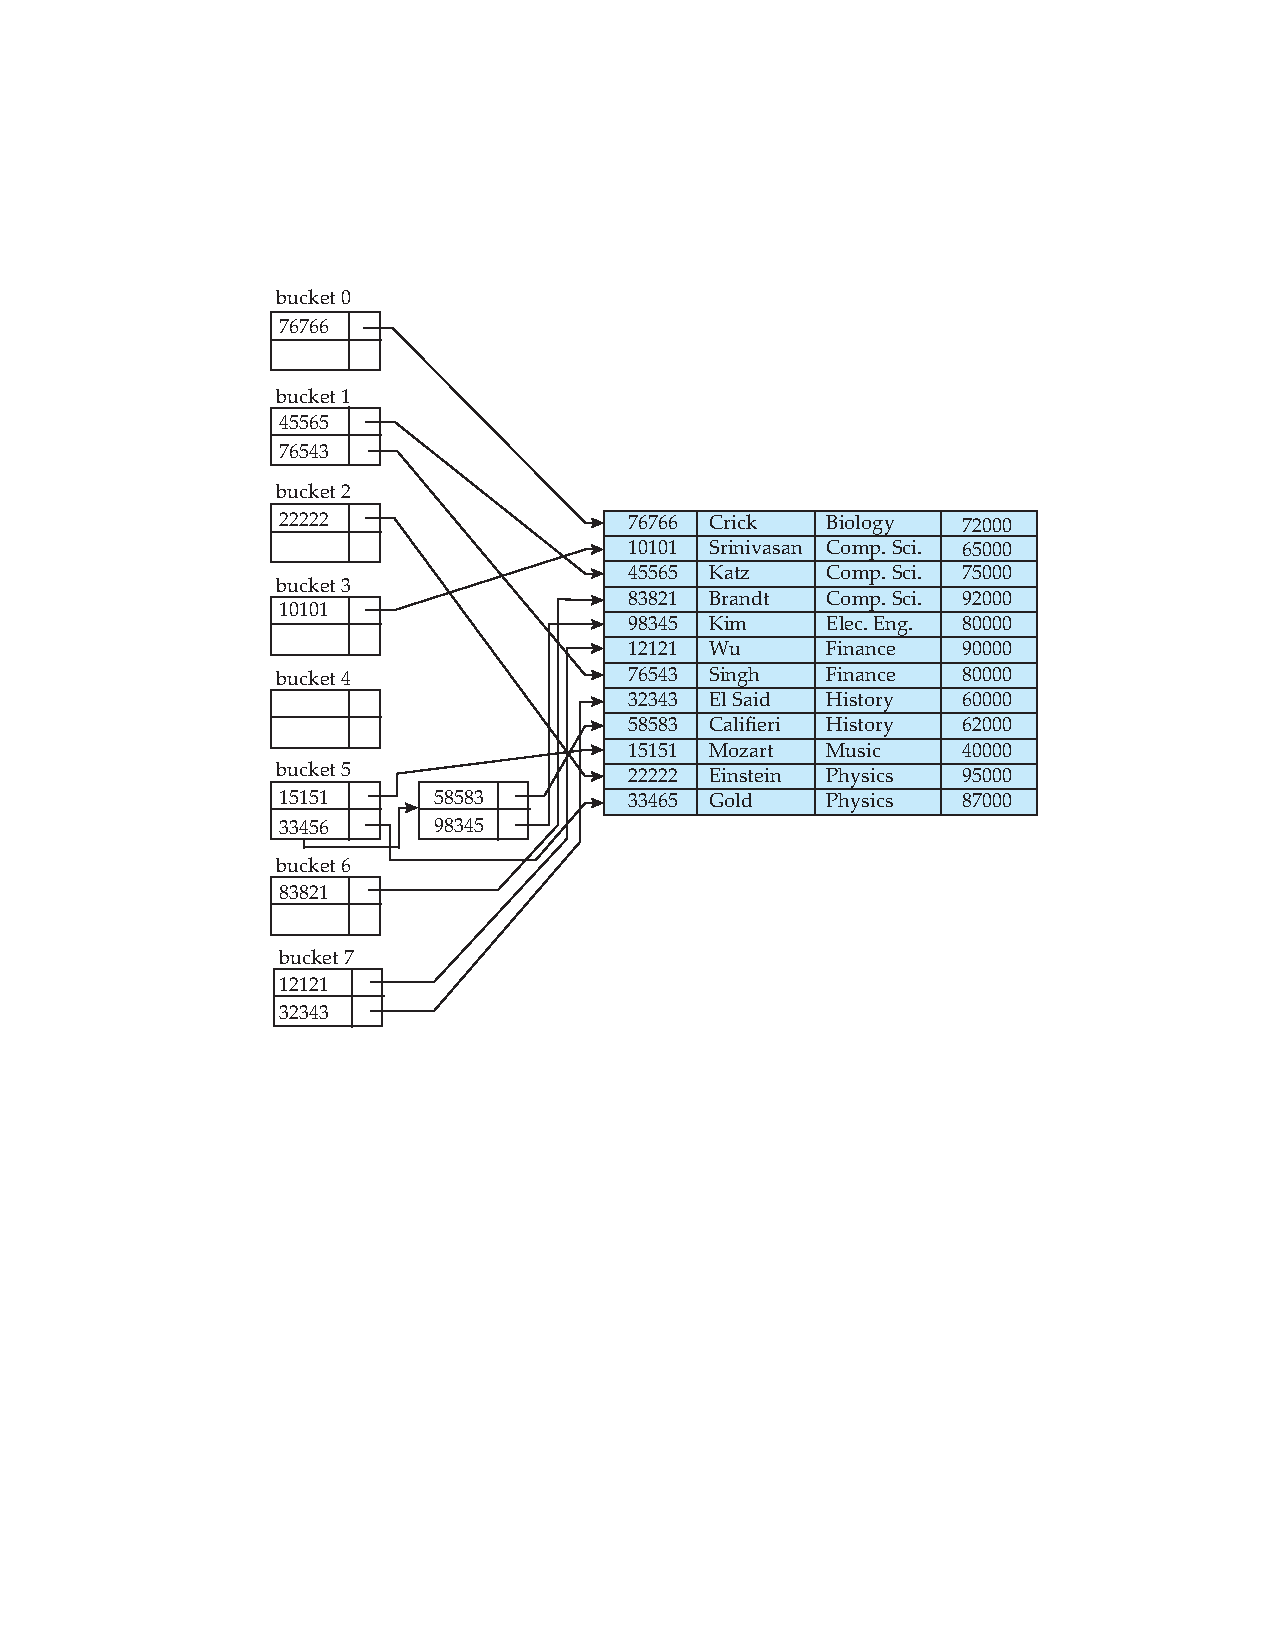
\includegraphics[width=.8\textwidth]{figure/散列索引.pdf}
    \caption{散列索引}
\end{figure}

\begin{lstlisting}[language=SQL, caption={MySQL中的散列索引}]
CREATE TABLE testhash (
    fname VARCHAR(50) NOT NULL,
    lname VARCHAR(50) NOT NULL,
    KEY USING HASH(fname)
) ENGINE=MEMORY;
\end{lstlisting}

B+树索引的索引: 当对某个页面访问次数满足一定条件时会将页
面地址存于Hash表, 下次查询时不需要B+树那样从根节点到叶
子节点逐级查找, 只需一次哈希算法即可立刻定位到相应的位置.


\subsection{位图索引}

\begin{itemize}
    \item 针对一些特殊的列建立索引;
    \item 列中的每一个值对应一个向量中的一位;
    \item 向量的长度对应于记录的条数;
    \item 不适合列中值的个数太多的情况.
\end{itemize}

\begin{figure}[H]
    \centering
    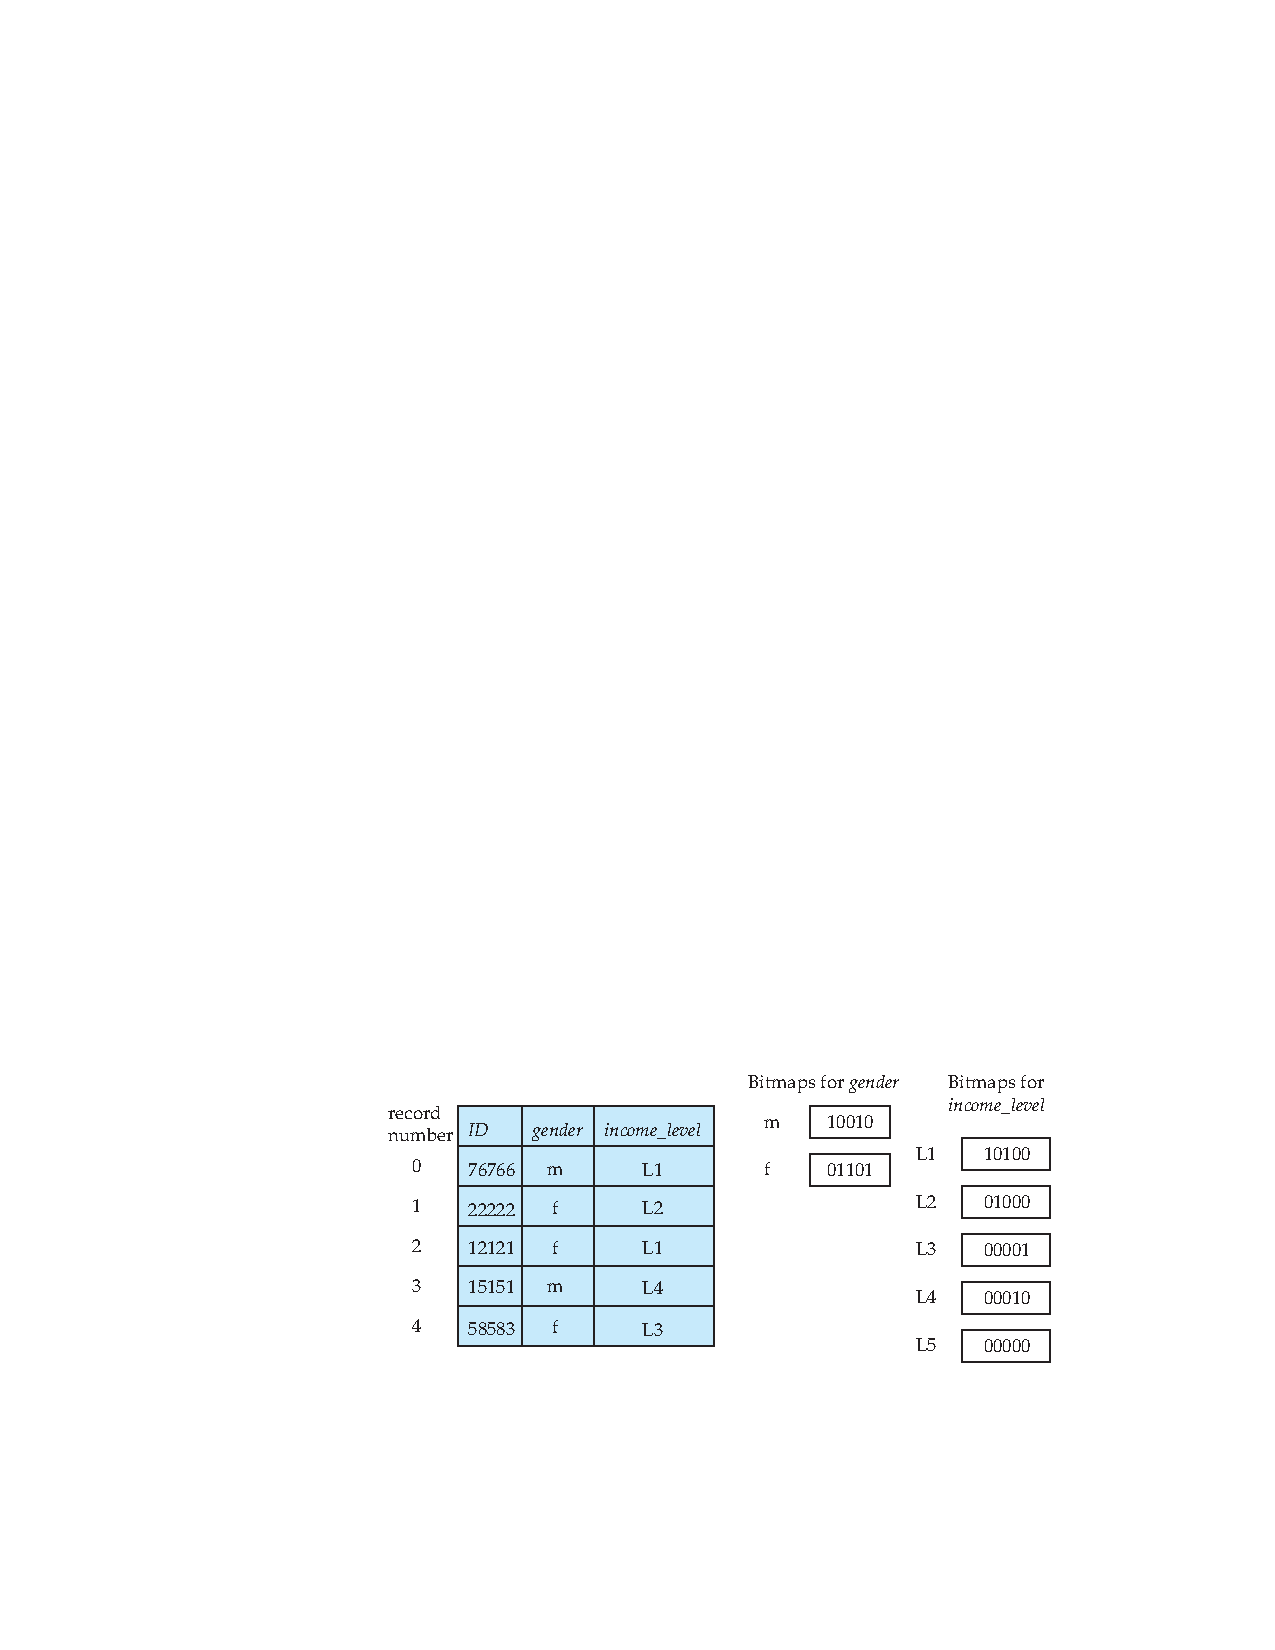
\includegraphics[width=.7\textwidth]{figure/位图索引.pdf}
    \caption{位图索引}
\end{figure}

现在我们考虑下面的查询:
\begin{lstlisting}[language=SQL]
select *
from instructor_info
where gender = 'f' and income_level = 'L2';
\end{lstlisting}

那么我们可以计算出gender值为'f'的位图和income\_level值为L2的位图的交(intersection)就能算出最终需要查询的记录.

\subsubsection{位片索引(Bit-sliced Index)}

位片索引是将属性列的域值按照某种方式进行垂直分割, 然后以二进制位图的形式存储.
\begin{figure}[H]
    \centering
    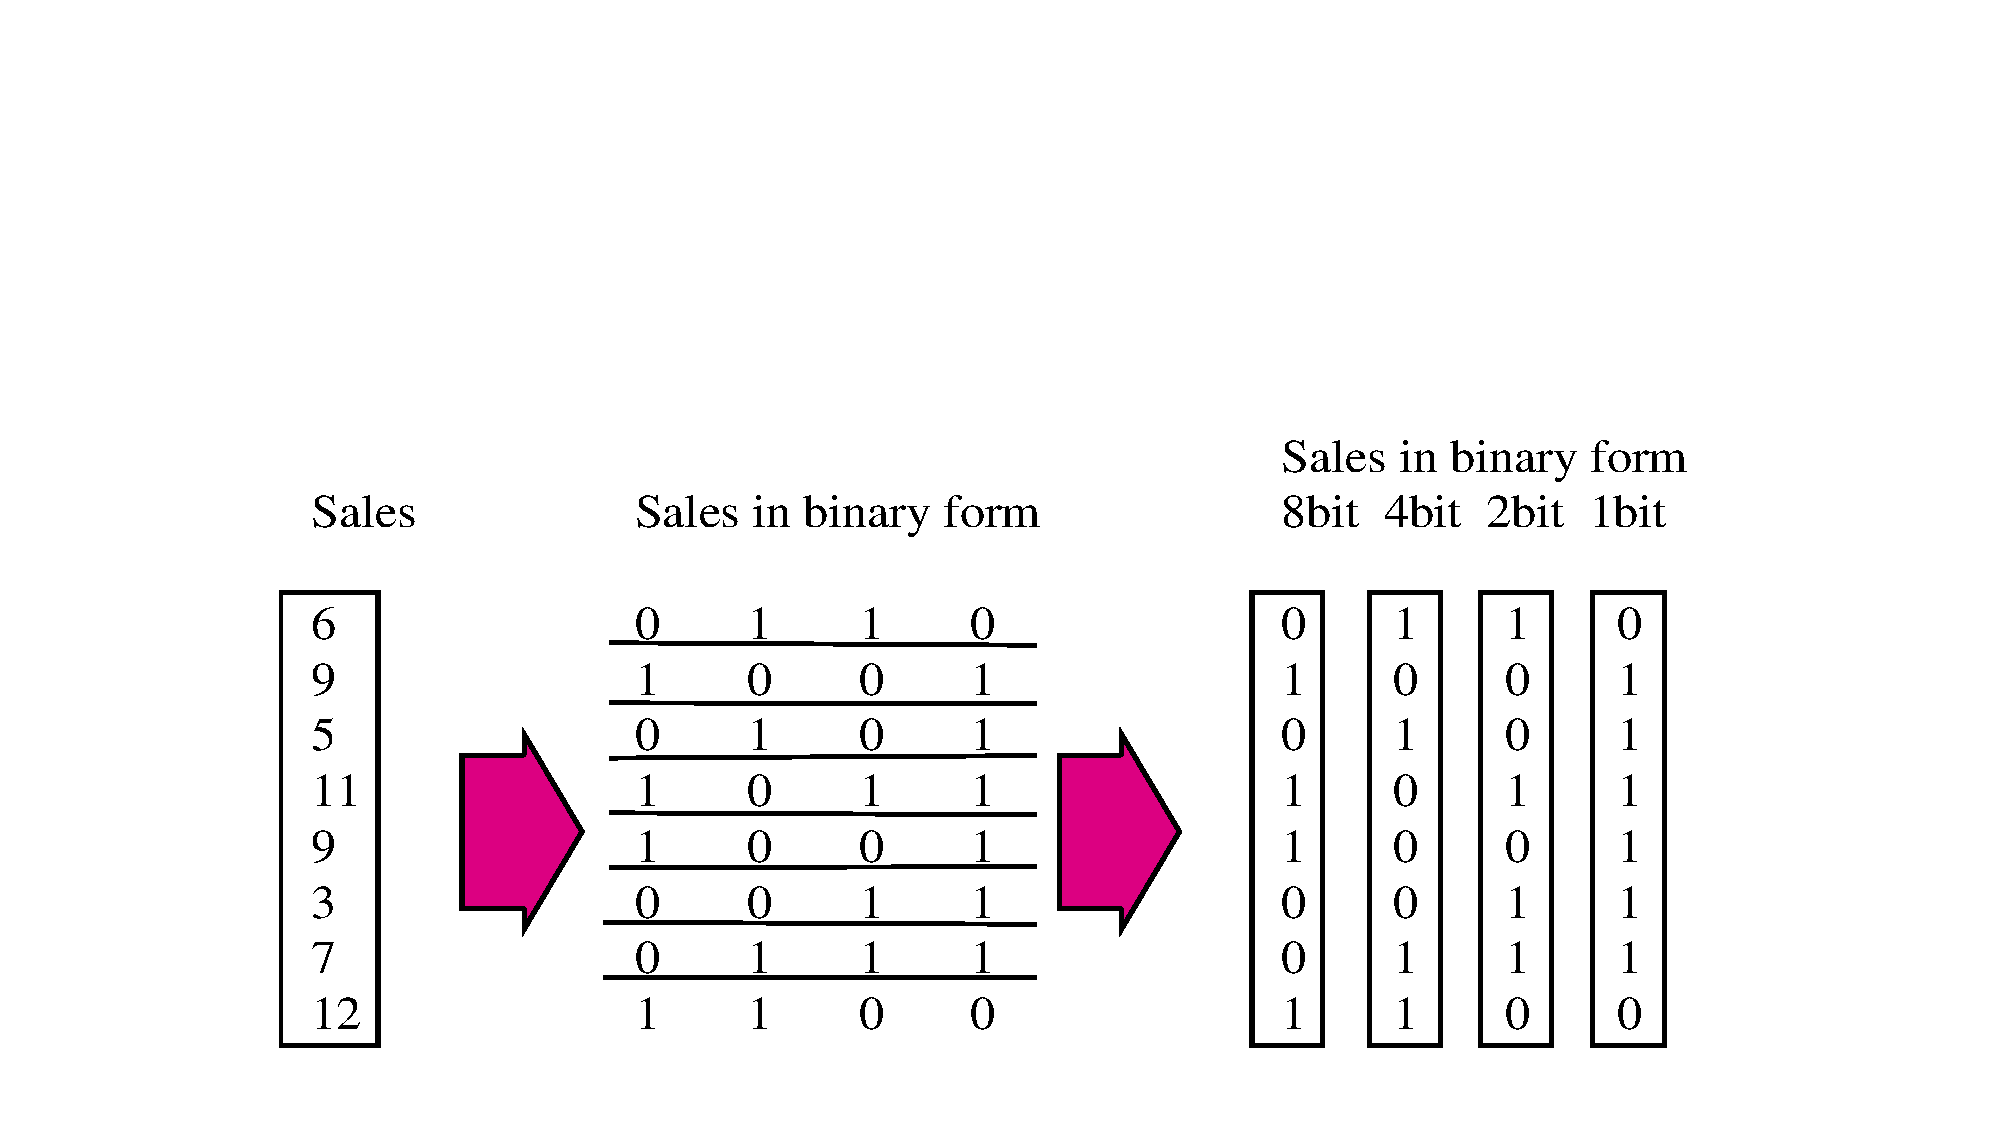
\includegraphics[width=.6\textwidth]{figure/位片索引.pdf}
    \caption{位片索引}
\end{figure}

\subsubsection{关系表的行式存储和列式存储}

行式存储的特点及其适合的场合:
\begin{itemize}
    \item 一条记录的所有字段存储在一起
    \item 各个字段的异质性导致压缩效果差
    \item 逻辑上访问单个字段, 物理上会把同一记录的其他字段一并返回
    \item 适合取回一条完整记录的场合(OLTP)
    \item 不适合针对单列的聚合分析(OLAP)
\end{itemize}

列式存储的特点:
\begin{itemize}
    \item 提高带宽利用率
    \item 提高数据压缩率: 将同一个属性域的数据存储在一起, 提高了局部性以及压缩比率. \textcolor{red}{宽表 + 稀疏表}.
    \item 增加插入操作的代价.
    \item 增加了磁盘寻道时间.
    \item 增加重构元组的代价.
\end{itemize}

列式存储的实现: MonetDB.

列式存储的实现: C-Store\cite{stonebrakerCstoreColumnorientedDBMS2018} \& Vertica\cite{lambVerticaAnalyticDatabase2012}.
\begin{itemize}
    \item 表被拆分成projections $\to$ Sales表被拆分成两个projections;
    \item 第一个projection按照date排序, 按照HASH(sale\_id)分段;
    \item 第二个projection按照cust排序, 按照HASH(cust)分段.
\end{itemize}

\begin{figure}[H]
  \centering
  \begin{minipage}[t]{0.32\textwidth}
    \centering
    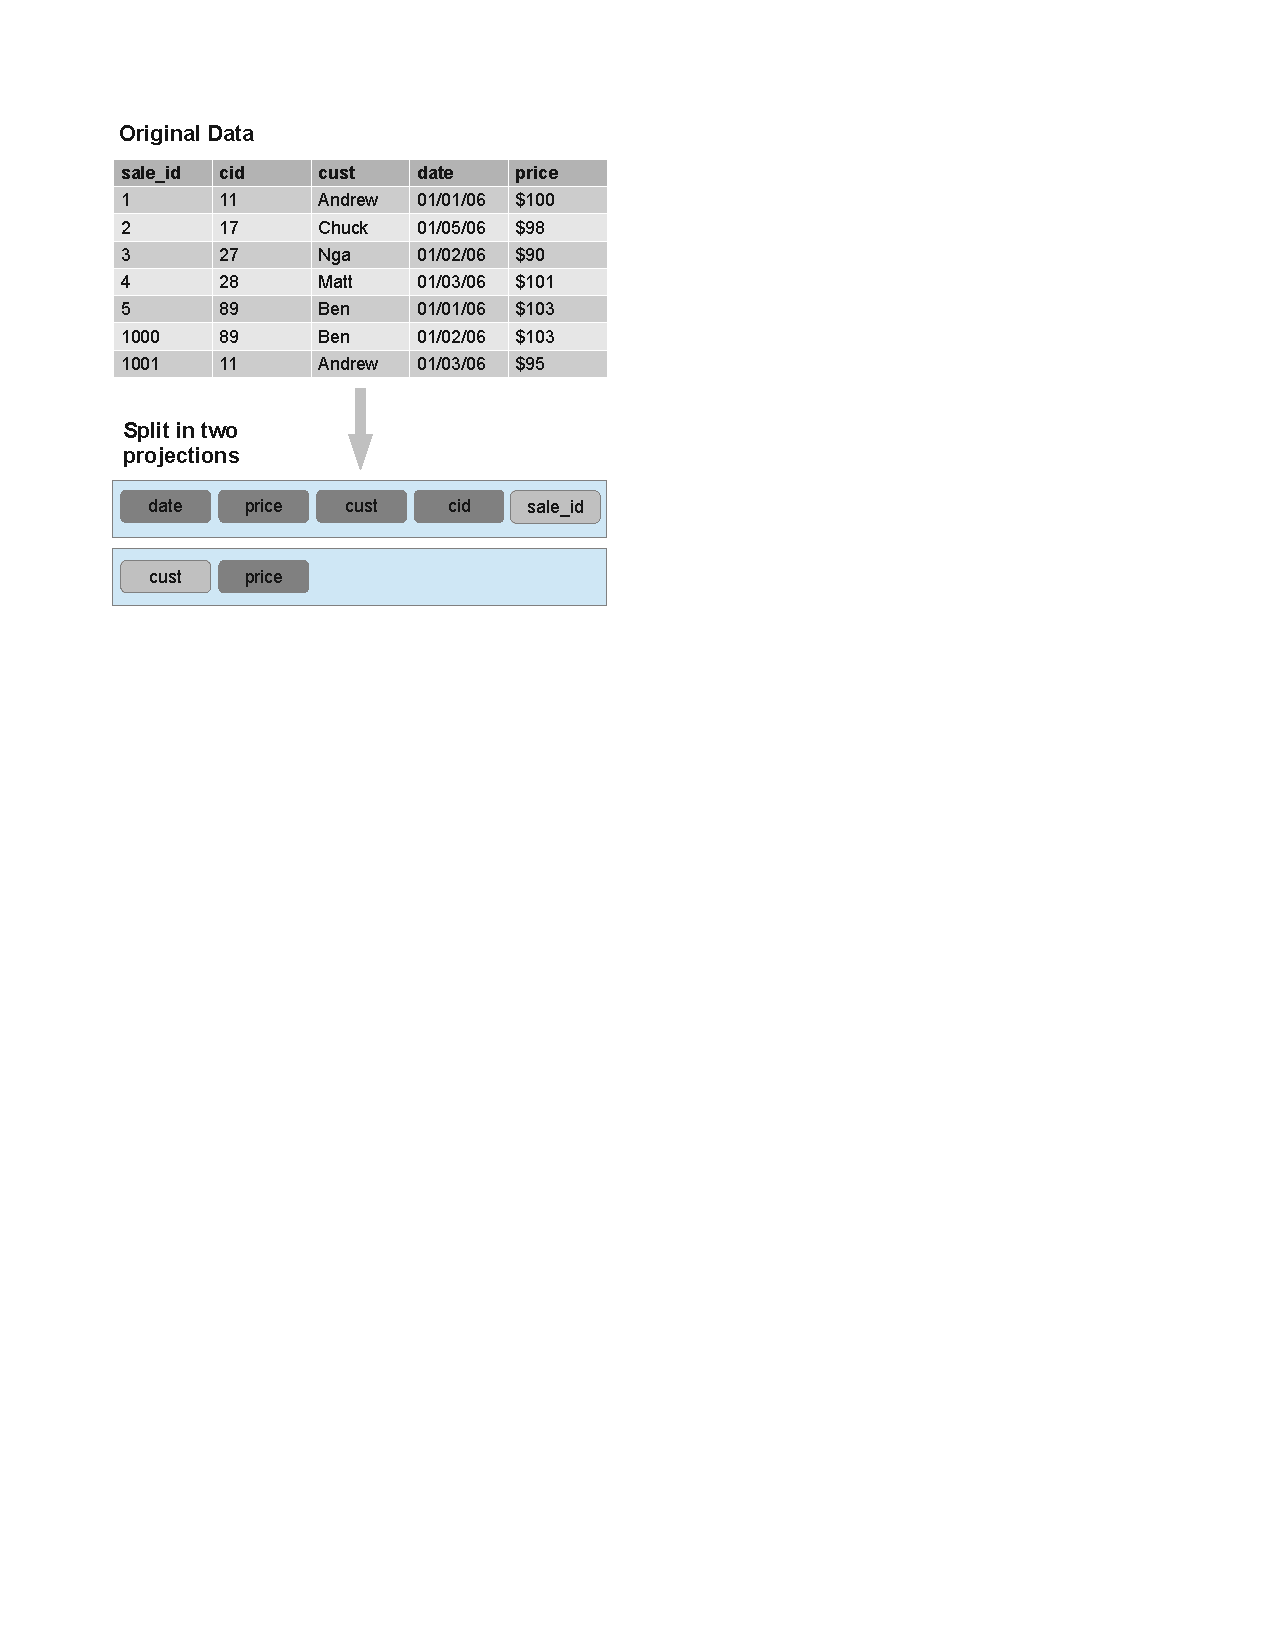
\includegraphics[width=\textwidth]{vertical-1.pdf}
  \end{minipage}
  \begin{minipage}[t]{0.34\textwidth}
    \centering
    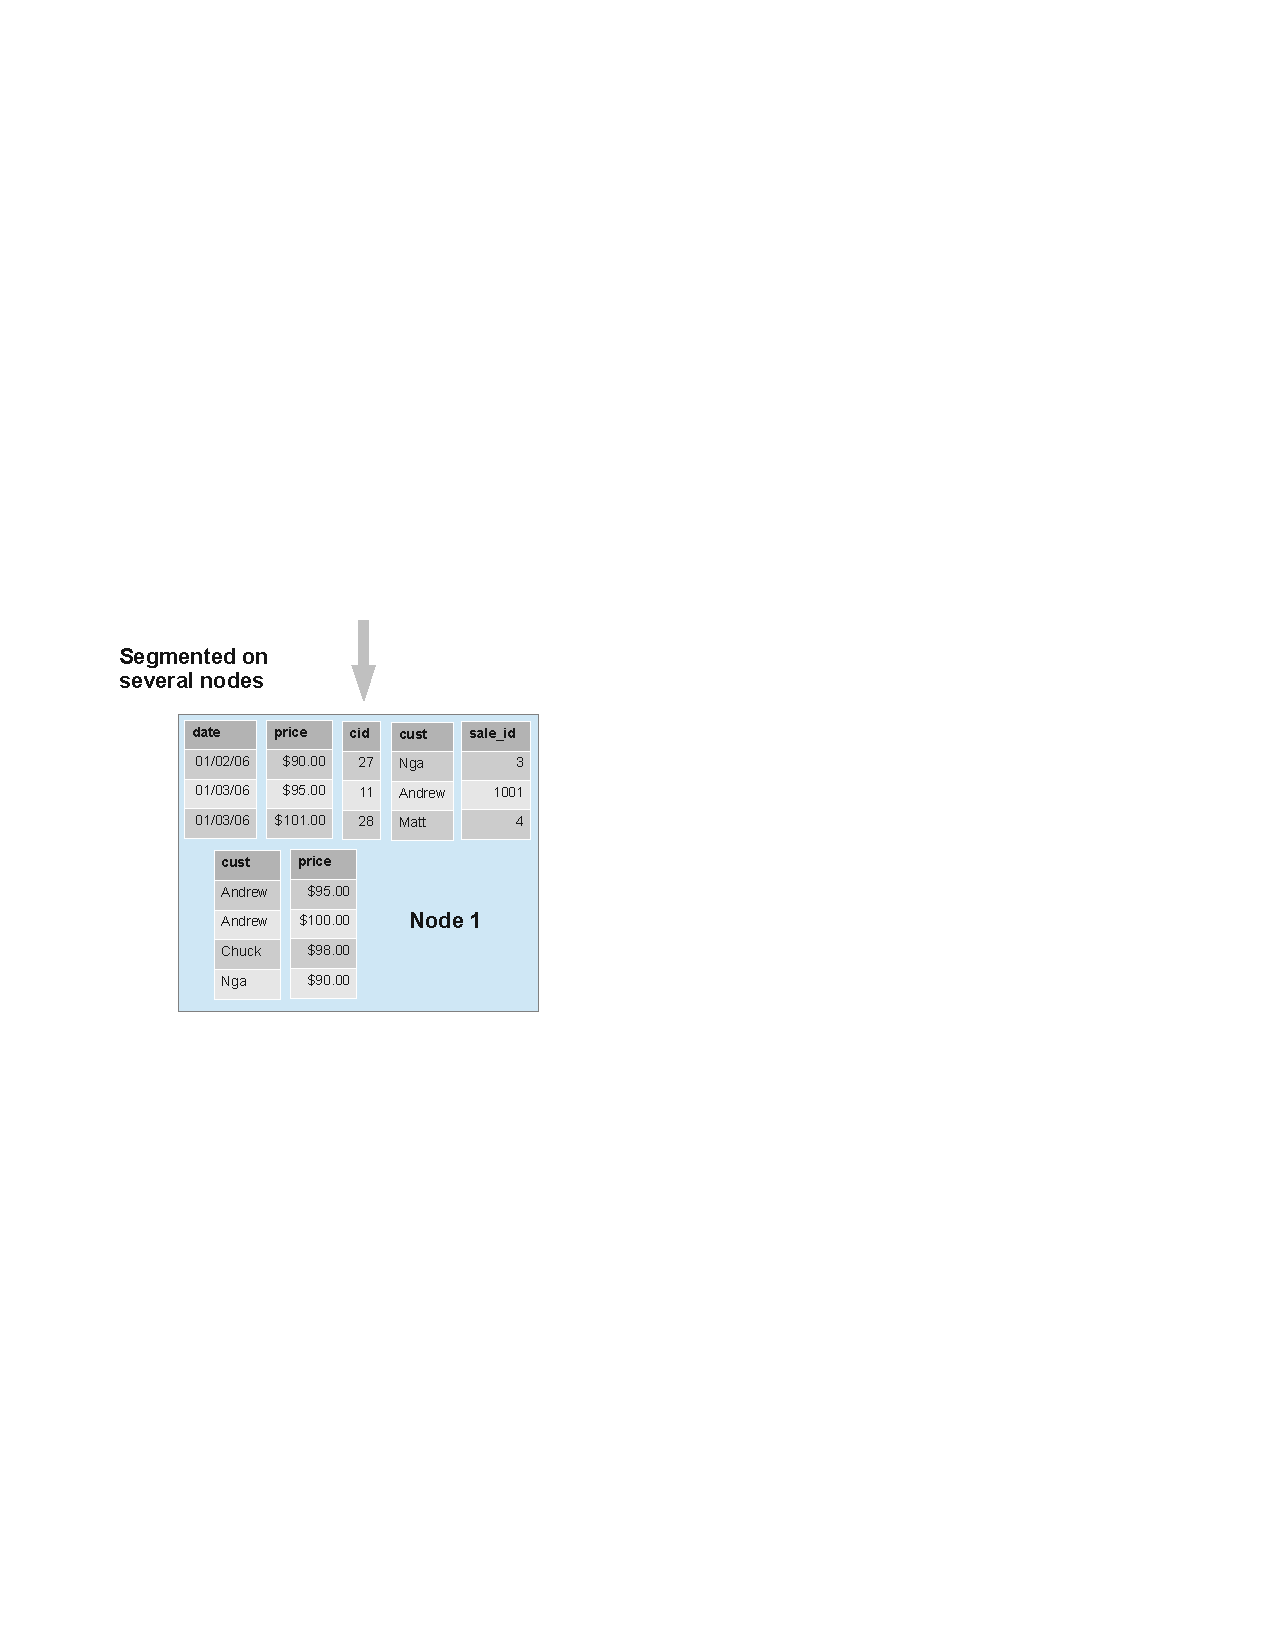
\includegraphics[width=\textwidth]{vertical-2.pdf}
  \end{minipage}
  \begin{minipage}[t]{0.3\textwidth}
    \centering
    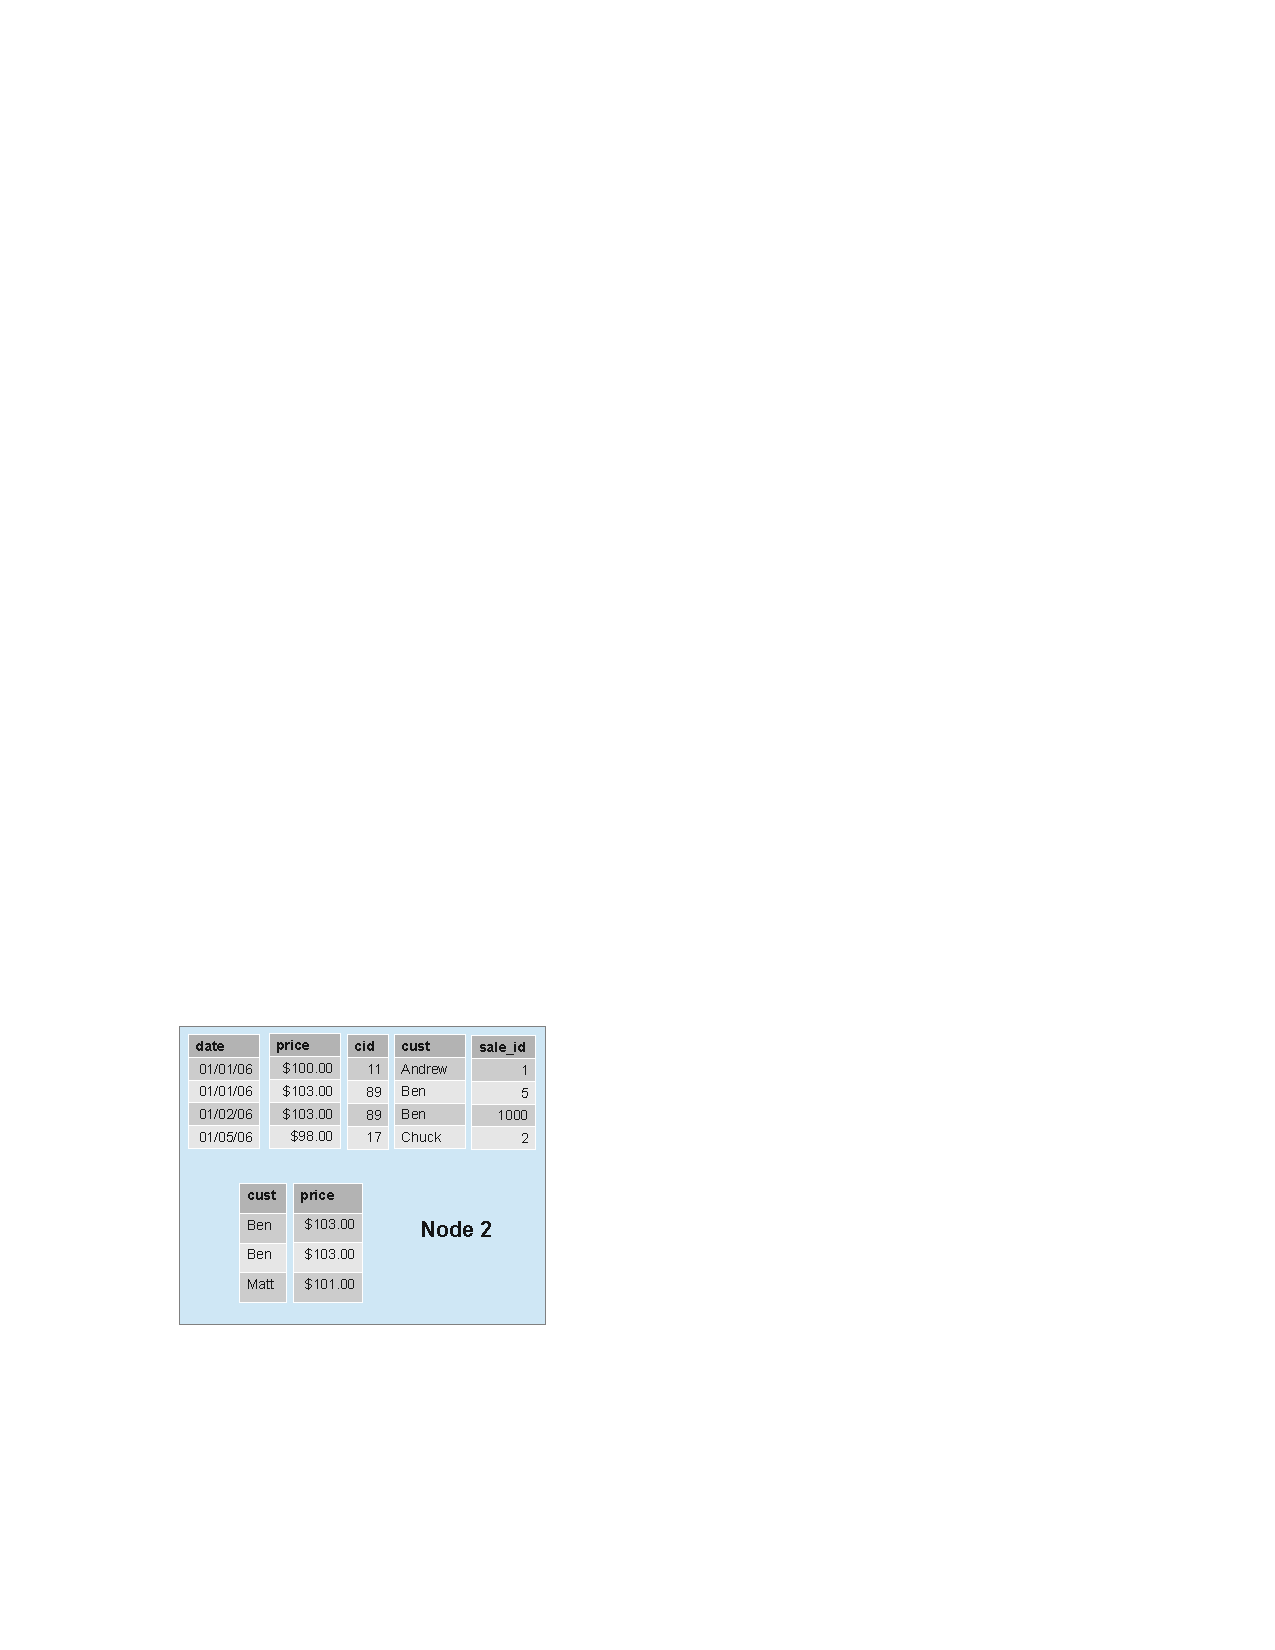
\includegraphics[width=\textwidth]{vertical-3.pdf}
  \end{minipage}
  \caption{Vertica的实现}
  \label{fig:three-side-by-side}
\end{figure}

稀疏属性可以压缩存储.

\subsection{多维索引}

多维索引的主要目的是为了加速对多维数据的检索速度, 例如范围查询(Range Query)和最近邻查询(Nearest Neighbor Query). 根据教材里的说法, 这是关于空间数据(Spatial Data)的存储的.
\begin{itemize}
    \item Nearest neighbor queries, given a point or an object, find the nearest object that satisfies given conditions.
    \item Range queries deal with spatial regions. e.g., ask for objects that lie partially or fully inside a specified region.
    \item Queries that compute intersections or unions of regions.
    \item Spatial join of two spatial relations with the location playing the role of join attribute.
\end{itemize}

\subsubsection{k-d tree}

早期用于多维索引的结构之一: k-d tree.

一棵 k-d 树的每一层都把空间分成两个部分, 在树顶层的节点处分区是沿着一个维度进行的, 在下一层节点中则沿着另一个维度进行. 分区的进行方式是这样的: 在每个节点处, 存储在子树中的大约一半的点落在一边且另一半落在另一边, 当一个节点的点数少于给定的最大点数时, 分区停止.

下面我们把叶节点中的最大点数被设置为1, 其中每条线对应于k-d树的一个节点, 线的编号表示相应节点出现在树中的层级.

比如说, 一个范围查询可能查找所有在$x$维度上是50到80, $y$维度是40到70. 可以通过以下递归过程来执行范围搜索:
\begin{enumerate}
    \item 假设节点是一个内部节点, 令它在点$x_i$处按一个特定维度(比如说$x$)被拆分. 左子树中的项所具有的$ x$值<$x_i$, 且右子树中的项所具有的$ x $值 $\geq x_i$. 如果查询范围包含$x_i$则在两个孩子上递归地执行搜索. 如果查询范围在$x_i$的左侧, 则只对左孩子执行递归搜索, 否则只在右子树上执行搜索.
    \item 如果节点是叶节点, 则检索查询范围中包含的所有项.
\end{enumerate}

\begin{figure}[H]
    \centering
    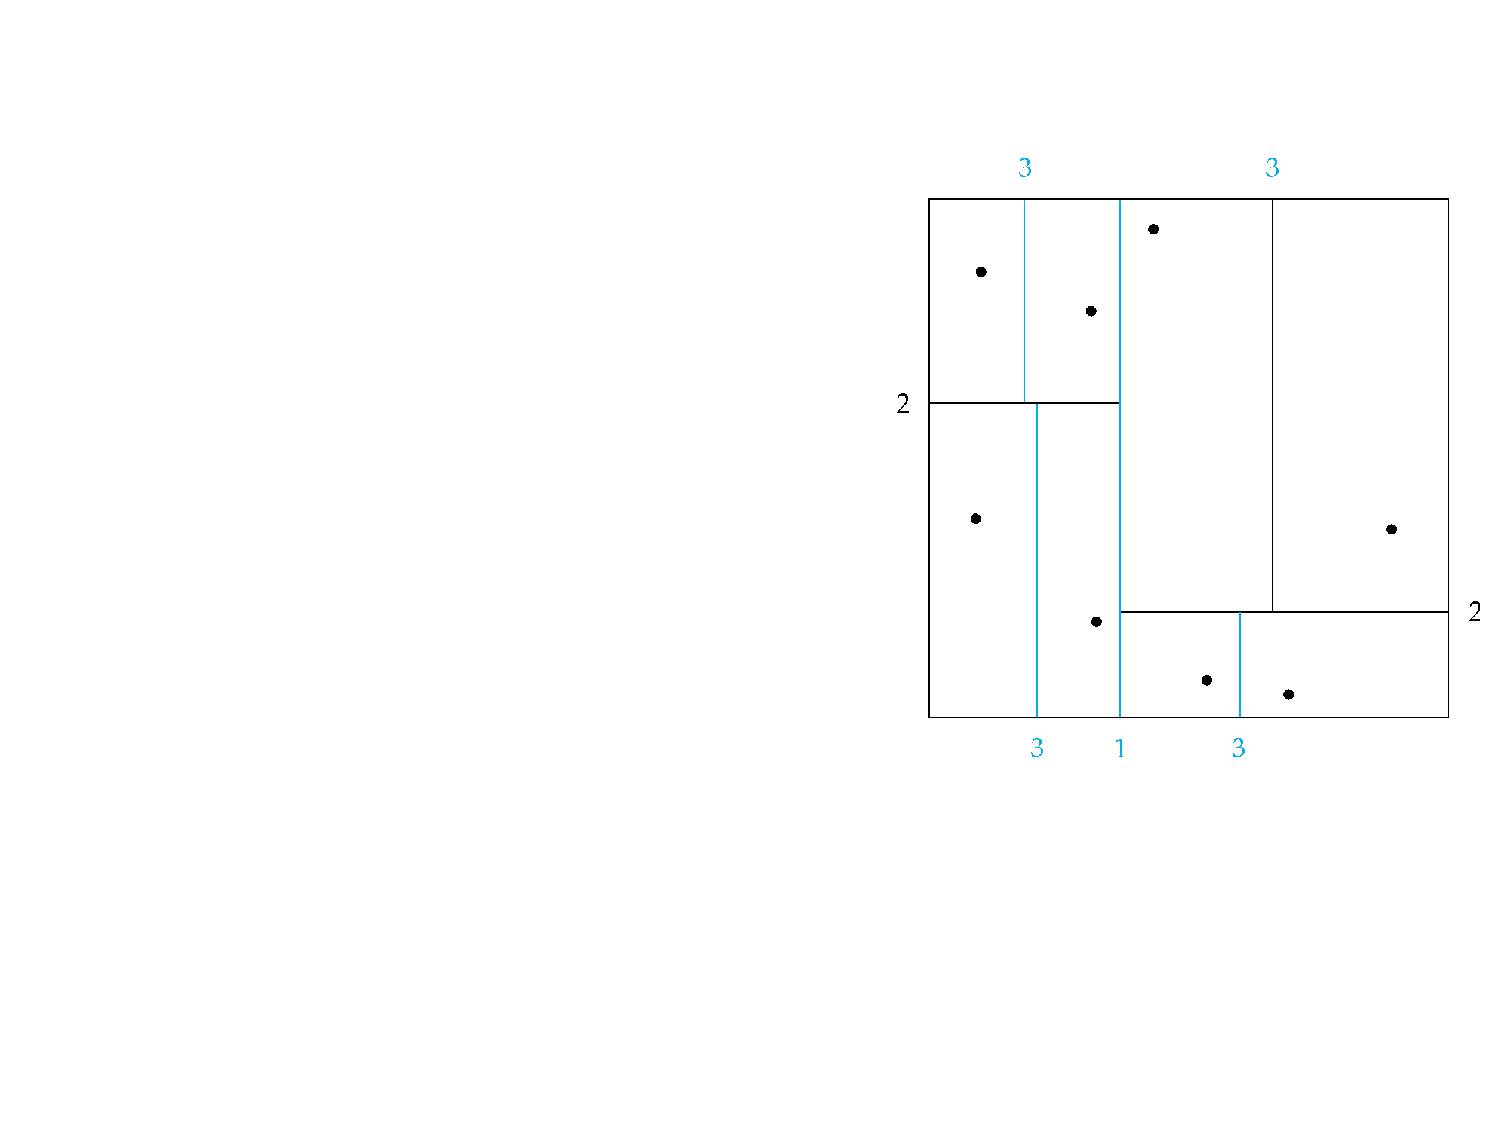
\includegraphics[width=.4\textwidth]{figure/k-d-tree.pdf}
    \caption{k-d树的例子}
\end{figure}

\subsubsection{四叉树}

四叉树(Quadtrees):
\begin{enumerate}
    \item 每个非叶子节点将其区域划分为四个大小相等的象限;
    \item 每个这样的节点都有四个子节点, 分别对应于这四个象限, 依此类推;
    \item 叶子节点的点数介于零到某个固定的最大点数之间(示例中设置为1).
\end{enumerate}

\begin{figure}[H]
    \centering
    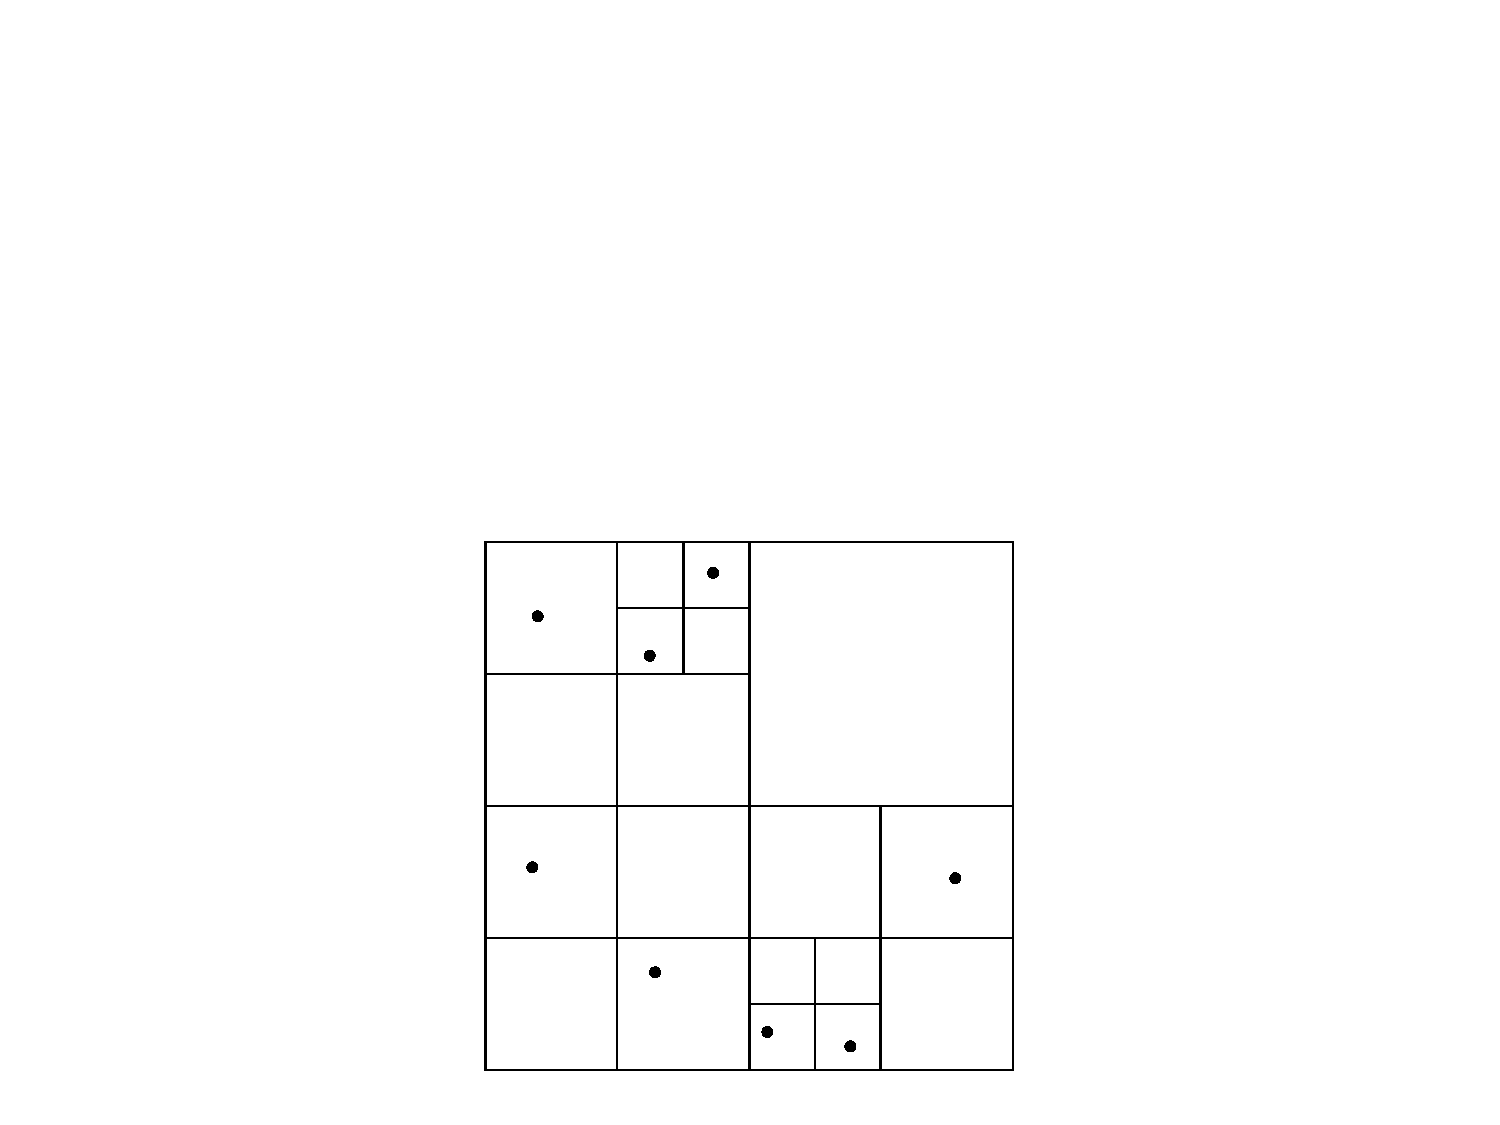
\includegraphics[width=.4\textwidth]{figure/四叉树.pdf}
    \caption{四叉树的例子}
\end{figure}

\subsubsection{R-tree}

一种称为 R 树 (R-tree) 的存储结构对于跨越空间区域的对象(比如线段、矩形和其他
多边形)以及点进行索引是有用的. R 树是一种平衡树结构, 索引对象存储在叶节点中, 这
很像 B+树. 但是, 与每个树节点关联的不是值的范围, 而是矩形边框 (bounding box). 叶
节点的边框是与包含叶节点中存储的所有对象的轴平行的最小矩形. 类似地, 内部节点的边
框是与包含其孩子节点边框的轴平行的最小矩形, 一个对象(比如多边形)的边框被类似地
定义为与包含该对象的轴平行的最小矩形.

每个内部节点存储孩子节点的边框以及指向孩子节点的指针. 每个叶节点存储被索引的对象. 下面的例子中边框$i$的坐标被标记为$BB_i$.
\begin{figure}[H]
    \centering
    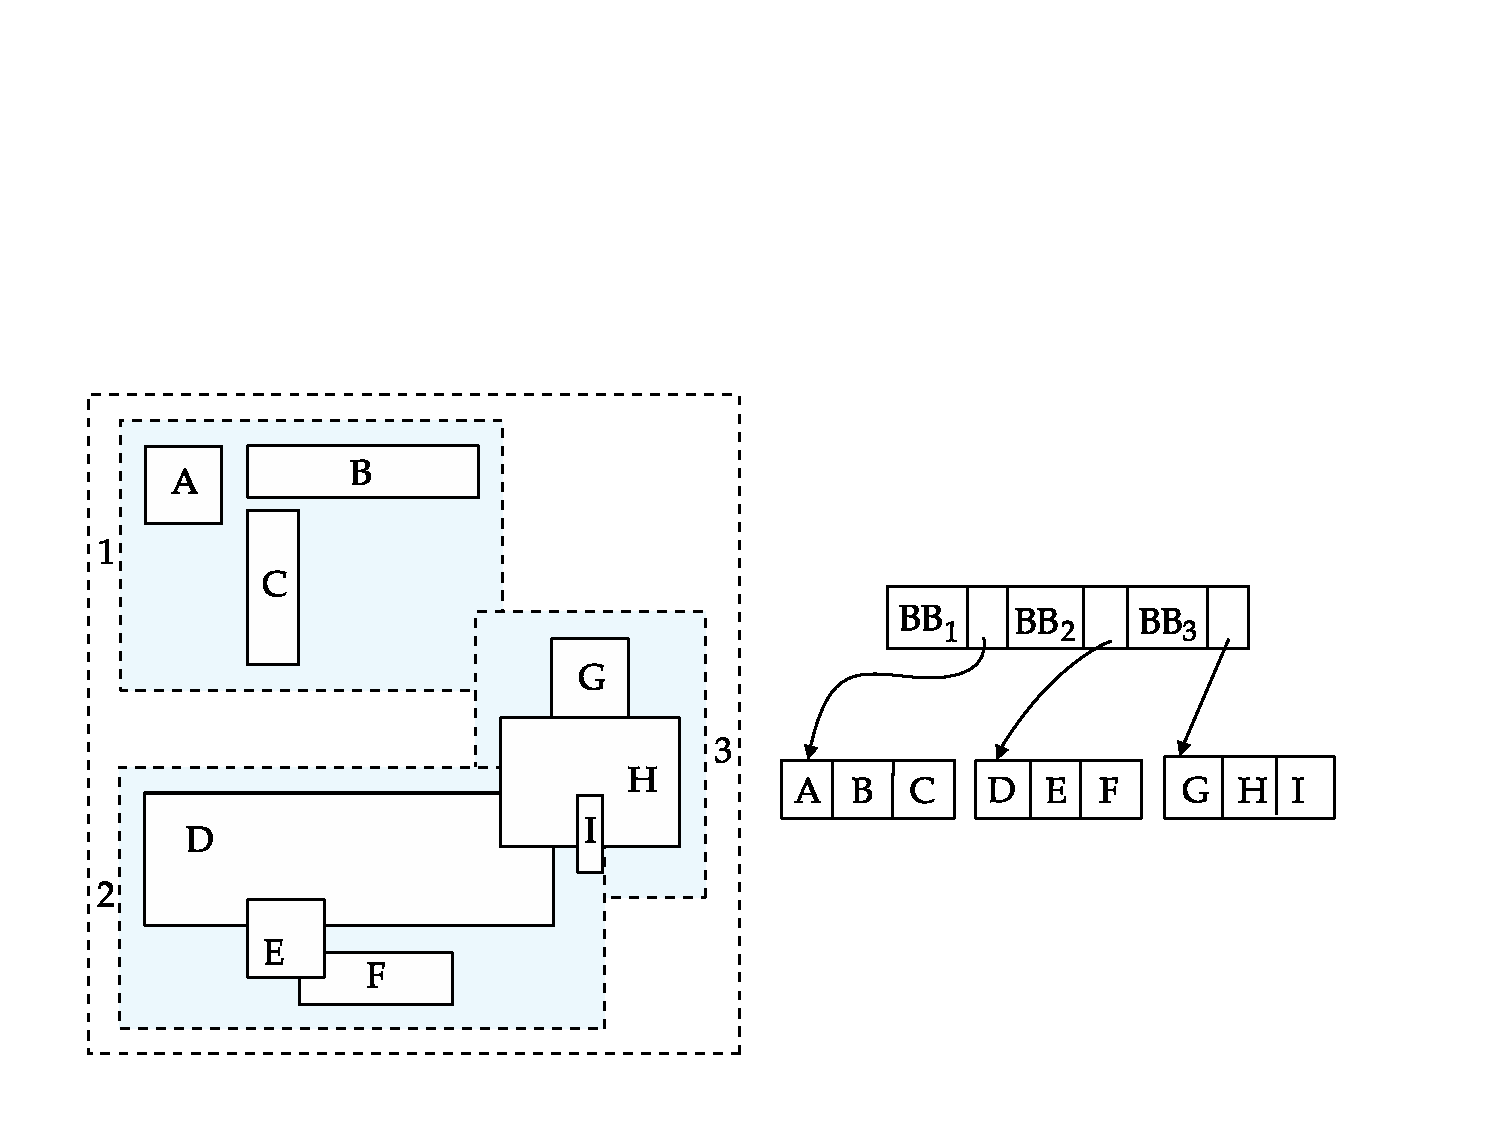
\includegraphics[width=.7\textwidth]{figure/R-tree.pdf}
    \caption{R树的例子}
\end{figure}

\subsection{LSM树}

LSM树(Log-structured merge tree): 写优化的索引结构. \cite{oneilLogstructuredMergetreeLSMtree1996}

\begin{itemize}
    \item 磁盘的顺序读性能远胜于随机读;
    \item B+树的读性能: \textcolor{red}{磁盘顺序读};
    \item B+树的写性能: \textcolor{red}{磁盘随机写}.
\end{itemize}

\subsubsection{LSM树的设计思想}

将$N$个数据划分成多个小的有序结构, 每$m$个数据在内存里排序一次, 这样就获
得$N/m$个有序结构; 查询时从最新的一个有序结构里做二分查找, 如果没找到就继
续查找下一个有序结构; 读取的时间复杂度是$N/m \times \log_2 N$

随着小树越来越大, 内存中的小树会flush到磁盘中, 磁盘中的树定期做merge
操作, 合并成一棵大树, 以优化读性能.

合并时, 不会像B+树一样, 在原数据的位置上修改, 而是直接
插入新的数据, 从而避免了随机写.

\textcolor{red}{LSM-Tree属于传输型, 因为它会使
用日志文件和一个内存存储结构把随机写操作转化为顺序写.}

\subsubsection{LSM树的增删查改}

LSM树结构横跨内存和磁盘, 包括:
\begin{itemize}
    \item memtable
    \item immutable memtable
    \item SSTable
\end{itemize}

\textbf{写入流程}:
\begin{enumerate}
    \item 来了一个$\text{put}(k,v)$操作, 首先追加到WAL日志中, 接下来加到C0层
    \item 当C0层的数据达到一定大小, 就把C0层和C1层合并
    \item 合并出来的新的new-C1会顺序写磁盘, 替换掉原来的old-C1
    \item 合并之后所有旧文件都可以删掉
\end{enumerate}

\textbf{删除操作}:
\begin{enumerate}
    \item 当有删除操作时, 并不需要像B树一样, 在磁盘中找到相应的数据后再删除, 只需要在memtable中插入一条数据当作标志, 如delKey:1933;
    \item 当读操作读到memtable中的这个标志时, 就会知道这个key已被删除;
    \item 在随后的\textcolor{red}{日志合并}中, 这条被删除的数据会在合并过程中一起被删除.
\end{enumerate}

\textbf{更新操作}:
\begin{enumerate}
    \item 和删除操作类似, 都是只操作memtable, 写入一个标志, 随后真正的更新操作被延迟在合并时一并完成.
\end{enumerate}

\begin{figure}[H]
    \centering
    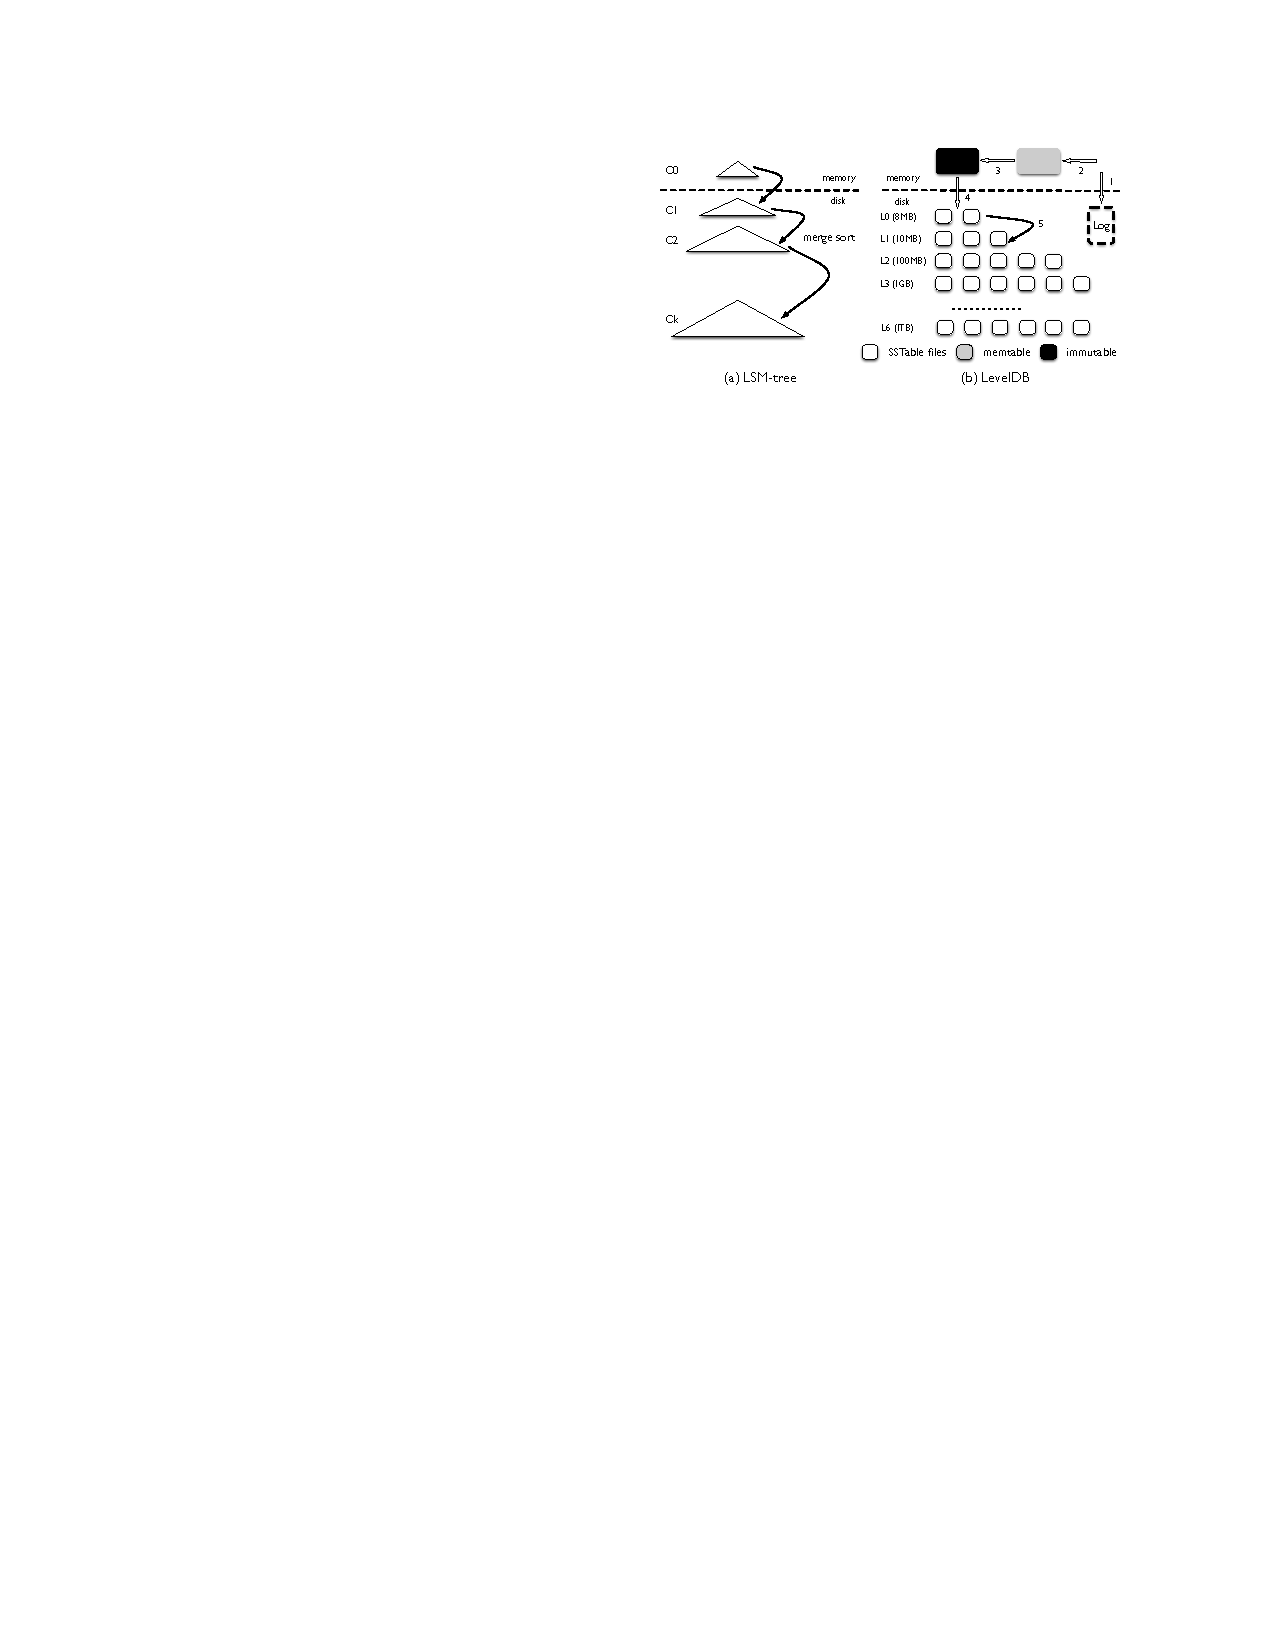
\includegraphics[width=.8\textwidth]{figure/LSM.pdf}
    \caption{LSM树的结构}
\end{figure}

\textbf{查询流程}:
\begin{enumerate}
    \item 读操作需要依次读取memtable、immutable memtable、SSTable0、SSTable1...
    \item 需要反序遍历所有的集合, 序号小的集合中的数据一定会比序号大的集合中的数据新
    \item 在这个反序遍历过程中一旦匹配到要读取的数据, 则一定是最新的数据, 返回该数据
    \item 对于不存在的数据, 则会白白遍历所有集合: 引入\textcolor{red}{布隆过滤器(Bloom Filter)}\footnote{操作系统的期末考试论文题也考到了.}来加速读操作, 当它显示相应的SSTable中没有要读取的数据时, 就跳过该SSTable.
\end{enumerate}

\textbf{Bloom Filter}: 其中有$m$个位, 使用$k$个hash functions $h_1,h_2,...,h_k$, 映射后的值范围为$\{1,...,m\}$.

\begin{figure}[H]
    \centering
    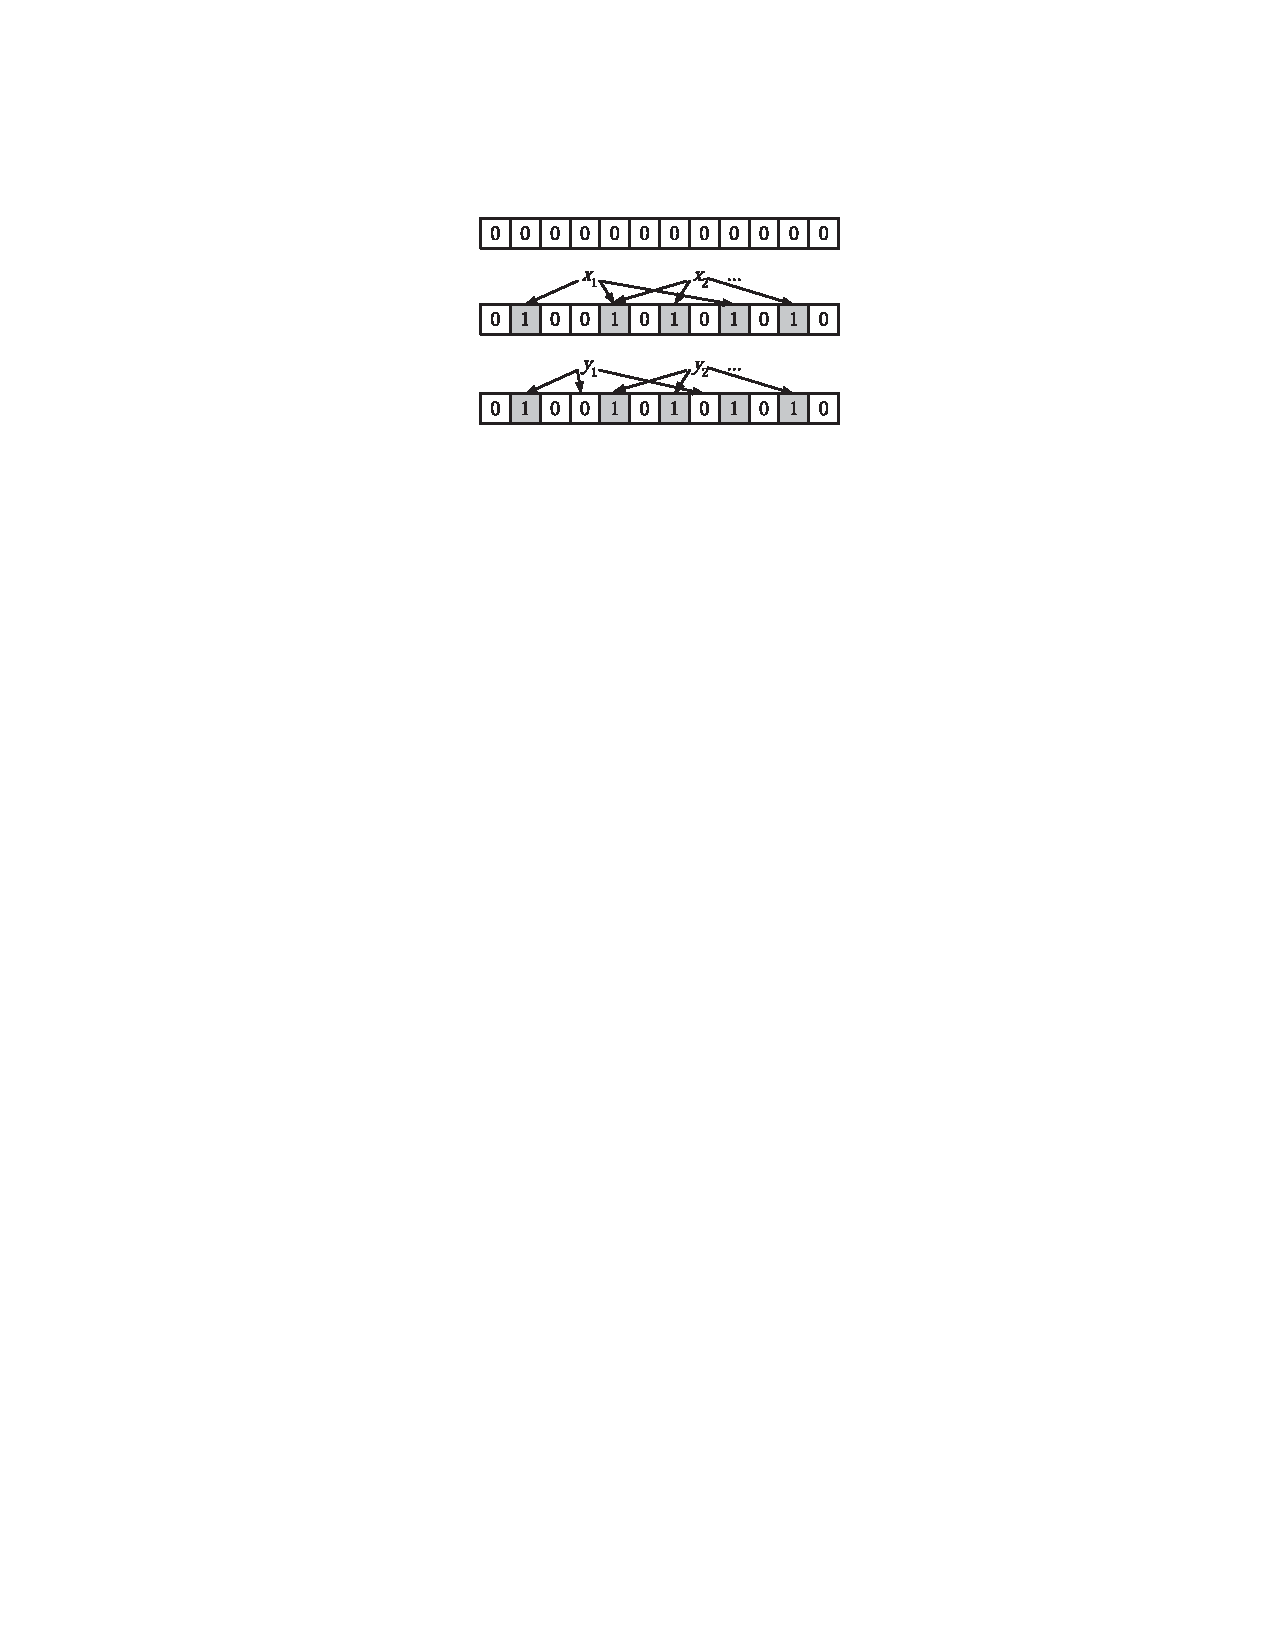
\includegraphics[width=.4\textwidth]{figure/bloom-filter.pdf}
    \caption{Bloom Filter的一个例子}
\end{figure}

如图, 我们先向集合里插入了$x_1$和$x_2$, 分别hash了$k$次, 对于得到的每个位置都设置为1.

接着, 我们试图查询$y_1$是否位于集合之中, 分别hash $k$次, 发现有位置是0, 这就意味着$y_1$肯定不在集合中(利用反证法, 假设在, 那么存在一个$x_t$使得$h_i(y_1)=h_i(x_t), i=1,2,...,k$, 这就意味着hash得到的位置应该都是1, 现在却反而有0, 矛盾!); 但是现在查询$y_2$, 发现hash的位置都是1了, 这就说明有可能在集合中, 也有可能不在.

\subsubsection{LSM-tree读写放大}

读写放大(read and write amplification)是 LSM-tree 的主要问题:
\begin{itemize}
    \item 读写放大 = 磁盘实际读写的数据量 / 用户访问的数据量
\end{itemize}

\begin{itemize}
    \item 以 Level Style Compaction机制为例, 它每次拿上一层的所有文件和下一层合并, 下一层大小是上一层的$ r $倍, 单次合并的写放大就是$r$倍;
    \item 假如现在有三层, 文件大小分别是: 9, 90, 900, $r=10$. 又写了个1, 这时就会不断合并, 1 + 9 = 10, 10 + 90 = 100, 100 + 900 = 1000, 总共写了10 + 100 + 1000.
    \item \textcolor{red}{读写放大 = 10/1 + 100/10 + 1000/100 = 30 = $r \times level$.}
\end{itemize}

\textcolor{red}{key-value越小读放大越大.}
\begin{itemize}
    \item 为了查询一个 1KB 的数据, 最坏需要读 L0 层的 8 个文件, 再读 L1 到 L6 的每一个文件, 一共 14 个文件;
    \item 而每个文件内部需要读16KB的索引, 4KB的布隆过滤器, 4KB的数据块, 一共 24 * 14 / 1 = 336倍.
\end{itemize}